\documentclass[12pt,twoside]{article}

% *** Set page dimensions ***
\raggedbottom
\parindent=0in
%\setlength{\topmargin}{-0.5in}
%\setlength{\oddsidemargin}{0.1875in}
%\setlength{\evensidemargin}{0in}
%\setlength{\textheight}{8.5in}
%\setlength{\textwidth}{6.225in}
%\addtolength{\oddsidemargin}{-0.7in}
%\addtolength{\evensidemargin}{-1.2in}
%\setlength{\oddsidemargin}{-0.2in}
%\setlength{\evensidemargin}{-0.2in}
%\addtolength{\textwidth}{1.4in}
%\addtolength{\topmargin}{-.875in}
%\addtolength{\textheight}{2.00in}

% *** Packages ***
\usepackage{alltt}
\usepackage{tocloft}
\usepackage{graphicx}
\usepackage{lscape}
\usepackage{amssymb}
\usepackage{float}
\usepackage{amsmath}
\usepackage{gensymb}
%\usepackage{subfigure}
\usepackage{lscape}
\usepackage{epsfig}
\usepackage{enumerate}
\usepackage{multicol}
\usepackage{fancyhdr}
\usepackage{epstopdf}
\usepackage{hyperref}
\usepackage{listings}

% *** Table of contents and Sectioning *** 
\setcounter{secnumdepth}{0}
\setcounter{tocdepth}{5}

% *** Table of contents and Sectioning *** 
\newcommand{\next}{\addtocounter{enumi}{9} \item}
\newcommand{\now}[1]{\setcounter{enumi}{#1}}
\newcommand{\Z}{\mbox{\sf Z\hspace{-1.5mm}Z}}
\newcommand{\R}{\mbox{\rm I\hspace{-0.75mm}R}}
\columnsep=0.75in

% *** Shortcuts for syntax ***
\newcommand{\ds}{\displaystyle }
\newcommand{\vsc}{\vspace{4mm}}
\newcommand{\dd}[1]{\frac{d}{d{#1}} \,} 
\newcommand{\ddx}{\frac{d}{dx} \,} 
\newcommand{\ddy}{\frac{d}{dy} \,} 
\newcommand{\ddz}{\frac{d}{dz} \,} 
\newcommand{\dydx}{\frac{dy}{dx} \,} 
\newcommand{\dydt}{\frac{dy}{dt} \,} 
\newcommand{\dfdx}{\frac{df}{dx} \,} 
\newcommand{\ddt}[1]{  \frac{d{#1}}{dt} }
\newcommand{\pp}[2]{  \frac{\partial{#1}}{\partial {#2}} }
\newcommand{\zx}{\frac{\partial z}{\partial x} \,}
\newcommand{\zy}{\frac{\partial z}{\partial y} \,}
\newcommand{\limh}{\lim_{h \rightarrow 0} \;}
\newcommand{\diff}{\frac{d}{dx} \,}
\newcommand{\de}{\Delta}
\renewcommand{\thesection}{\Roman{section}}
\newcommand{\bfr}{\begin{flushright}}
\newcommand{\efr}{\end{flushright}}
\newcommand{\dx}{\frac{\partial f}{\partial x} \,}
\newcommand{\dy}{\frac{\partial f}{\partial y} \,}
\newcommand{\p}{\partial}
\newcommand{\vi}{\vec{i}}
\newcommand{\vj}{\vec{j}}
\newcommand{\vk}{\vec{k}}
\newcommand{\lan}{\left\langle}
\newcommand{\ran}{\right\rangle}
\newcommand{\reading}[1] { {\em Reading: #1}}
\renewcommand{\Pr}{ \mbox{Pr}}

% *** Commands related to textbook references
\newcommand{\problem}{{\bf Problem.} }

% *** Footnoting with symbols ***
\long\def\symbolfootnote[#1]#2{\begingroup%
\def\thefootnote{\fnsymbol{footnote}}\footnote[#1]{#2}\endgroup}

% *** Defining a boxed note ***
\floatstyle{boxed}
\newfloat{noteinbox}{htb}{loa}
\newenvironment{boxnote}{\begin{noteinbox}[H]}{\end{noteinbox}}

\newcommand{\Question}{ {\bf Question: }  }
\newcommand{\Example}[1]{ {\bf Example: } {\em #1} }
\newcommand{\ExampleCont}[1]{ {\em #1} }

% *** Define the boxed Week #/summary at the beginning/end of every chapter ***
\newcommand{\sectionbox}[1]{% 
\begin{tabular}{|p{6in}|}%
\hline%
\ \\ %
{\Large {\bf {#1}}}  \\%
\ \\%
\hline%
\end{tabular}}

% *** Shortcuts *** 
\newcommand\goals{\large {\bf {Goals:}}}
\newcommand\setfont{ }

% *** Week commands: overwritten in each notes file
\newcommand{\Week}{Null-InPreambleCommon}
\newcommand{\WeekTitle}{Null-InPreambleCommon}
\newcommand{\Course}{MNTC P04}
\newcommand{\SetNum}{1 }
\newcommand{\topic}[1]{
\newpage
\setcounter{page}{1}
\fancyhead[LE,RO]{#1 - \thepage}
}

% *** Setup Latex for the large version of the files ***
%\usepackage[landscape]{geometry}
\usepackage[letterpaper,landscape,hmargin={.8in,.8in},vmargin={1in,0.2in}]{geometry}

% Remove paragraph indents
\setlength{\parindent}{0pt}

% Spacing at the top for the header is too large by default
\setlength{\voffset}{-5ex}

% **** RENEW SCALING COMMANDS HERE ****
% *** Text in boxes ***
\renewenvironment{boxnote}{\begin{noteinbox}[H] \huge}{\end{noteinbox}} 

% *** Chapter lead in/summary boxes ***
\renewcommand{\sectionbox}[1]{% 
\begin{tabular}{|p{9.5in}|}%
\hline%
\ \\ %
{\huge {\bf {#1}}}  \\%
\ \\%
\hline%
\end{tabular}}

% *** 'Section'' commands, which are sometimes used for spacing
% From http://zoonek.free.fr/LaTeX/LaTeX_samples_section/0.html
\makeatletter
 \renewcommand\section{\@startsection {section}{1}{\z@}%
                                    {-3.5ex \@plus -1ex \@minus -.2ex}%
                                    {0.3ex \@plus.2ex}%
                                    {\setfont\bf}}

 \renewcommand\subsection{\@startsection {subsection}{1}{\z@}%
                                    {-3.5ex \@plus -1ex \@minus -.2ex}%
                                    {0.3ex \@plus.2ex}%
                                    {\setfont\bf}}

% *** 'Goals' should be larger in the overheads ***
\renewcommand\goals{\huge {\bf {Goals:}}}
\renewcommand\setfont{\huge }

\thispagestyle{empty}

\setfont 

\newcommand{\WeekTitleOne}{Derivatives - Foundations}
\newcommand{\WeekTitleTwo}{Derivatives - Linearization and Applications}
\newcommand{\WeekTitleThree}{Derivatives - Modeling}
\newcommand{\WeekTitleFour}{Integrals - Foundations}
\newcommand{\WeekTitleFive}{Integrals - Techniques}
\newcommand{\WeekTitleSix}{Integrals - Modeling}
\newcommand{\WeekTitleSeven}{Differential Equations - }
\newcommand{\WeekTitleEight}{Differential Equations - }
\newcommand{\WeekTitleNine}{Differential Equations - }
\newcommand{\WeekTitleTen}{Linear Algebra - }
\newcommand{\WeekTitleEleven}{Linear Algebra - }
\newcommand{\WeekTitleTwelve}{Linear Algebra - }



\begin{document}
\setfont
\pagestyle{fancy}
\renewcommand{\Week}{6 }
\renewcommand{\WeekTitle}{\WeekTitleSix }

\fancyhead[LE,RO]{Week \Week}  % default, usually only for first page
\fancyfoot{}
\sectionbox{Week \#\Week: \WeekTitle}


\vspace{5mm}
\goals
\begin{itemize}
\item Use MATLAB to solve a variety of integration problems. 
\item Use integration to find the average value of a function.
\item Use MATLAB to find the average value of a function. 
\item Use MATLAB to find the average value of a sequence of data. 
\end{itemize}
\vspace{5mm}


\topic{Numerical Integration - Motivation}
\subsection*{Numerical Integration - Motivation}
A common engineering challenge is to transfer heat generated by a
motor or combustion into a nearby fluid.

This transfer is often made more effective by the use of {\bf cooling
  fins}, which increase the surface area of contact with the fluid.

\begin{center}
  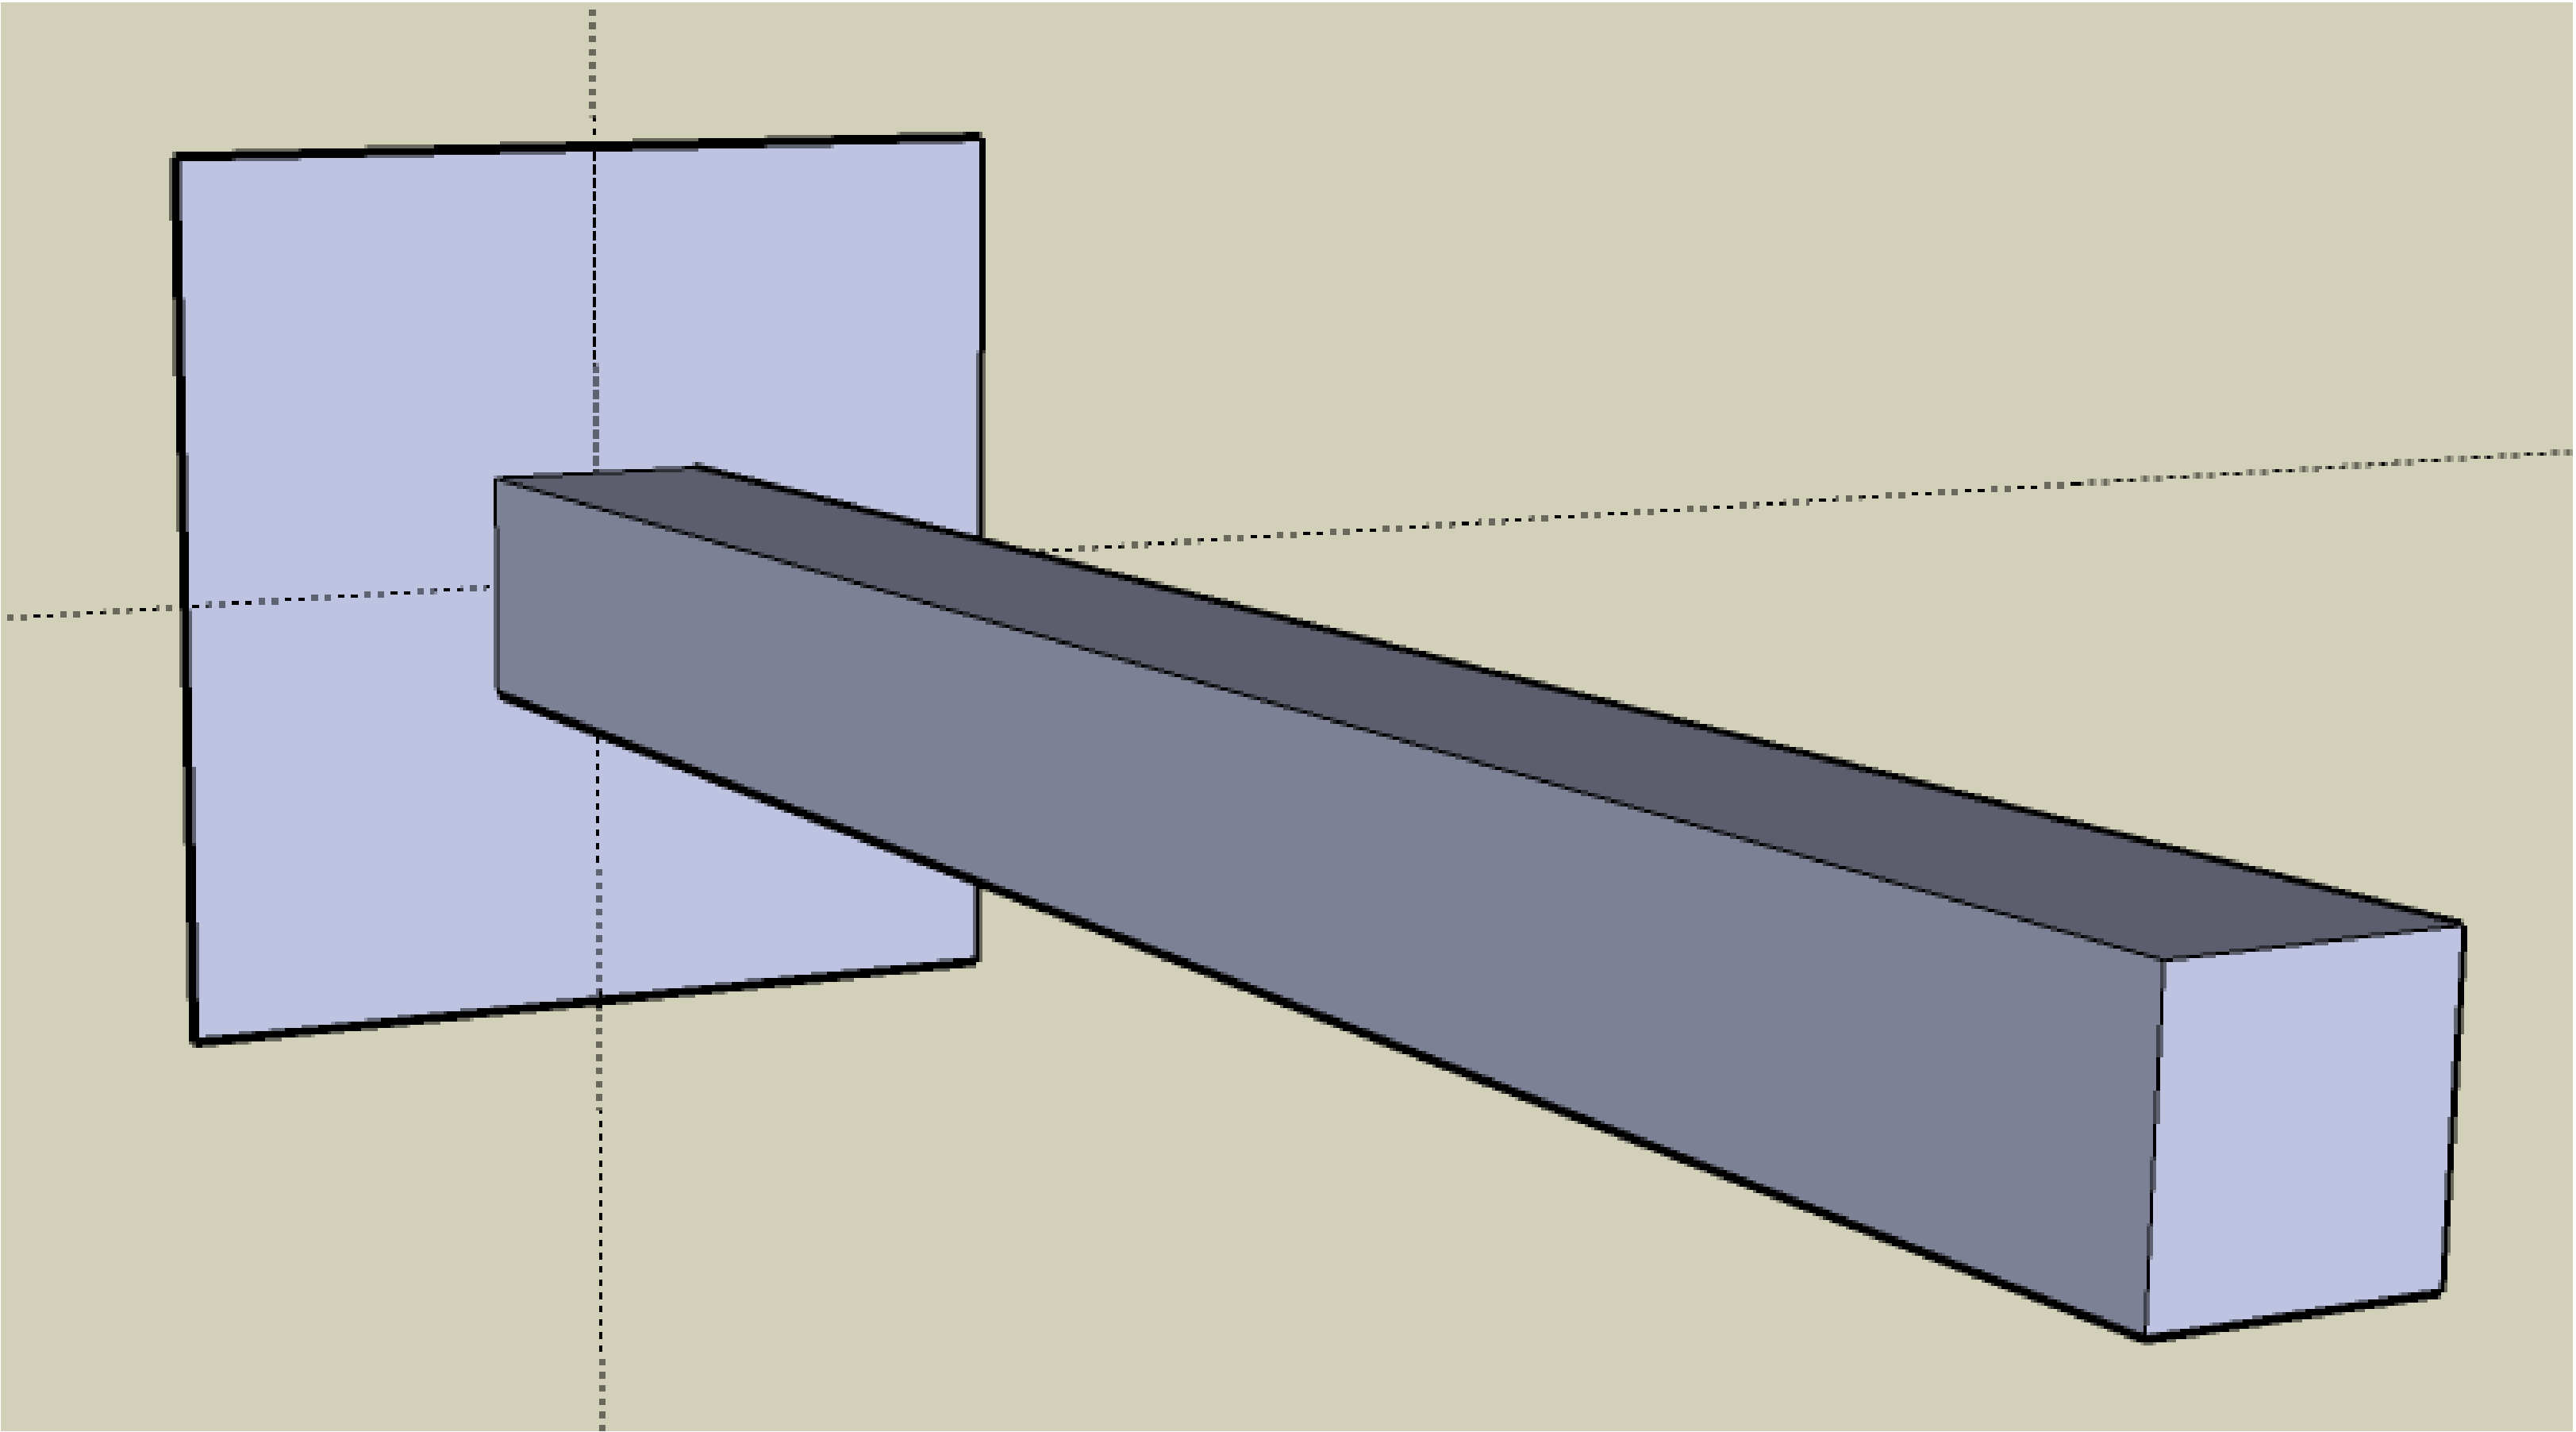
\includegraphics[width=5in]{graphics/notes_06_LongPin3D}
\end{center}

If we fix the temperature at the base, we can ask the question \\
{\bf ``How quickly is heat radiated out of fin?''}

\newpage
\vsc
\problem What factors affect the rate of heat transfer out of the
  fin?

\begin{center}
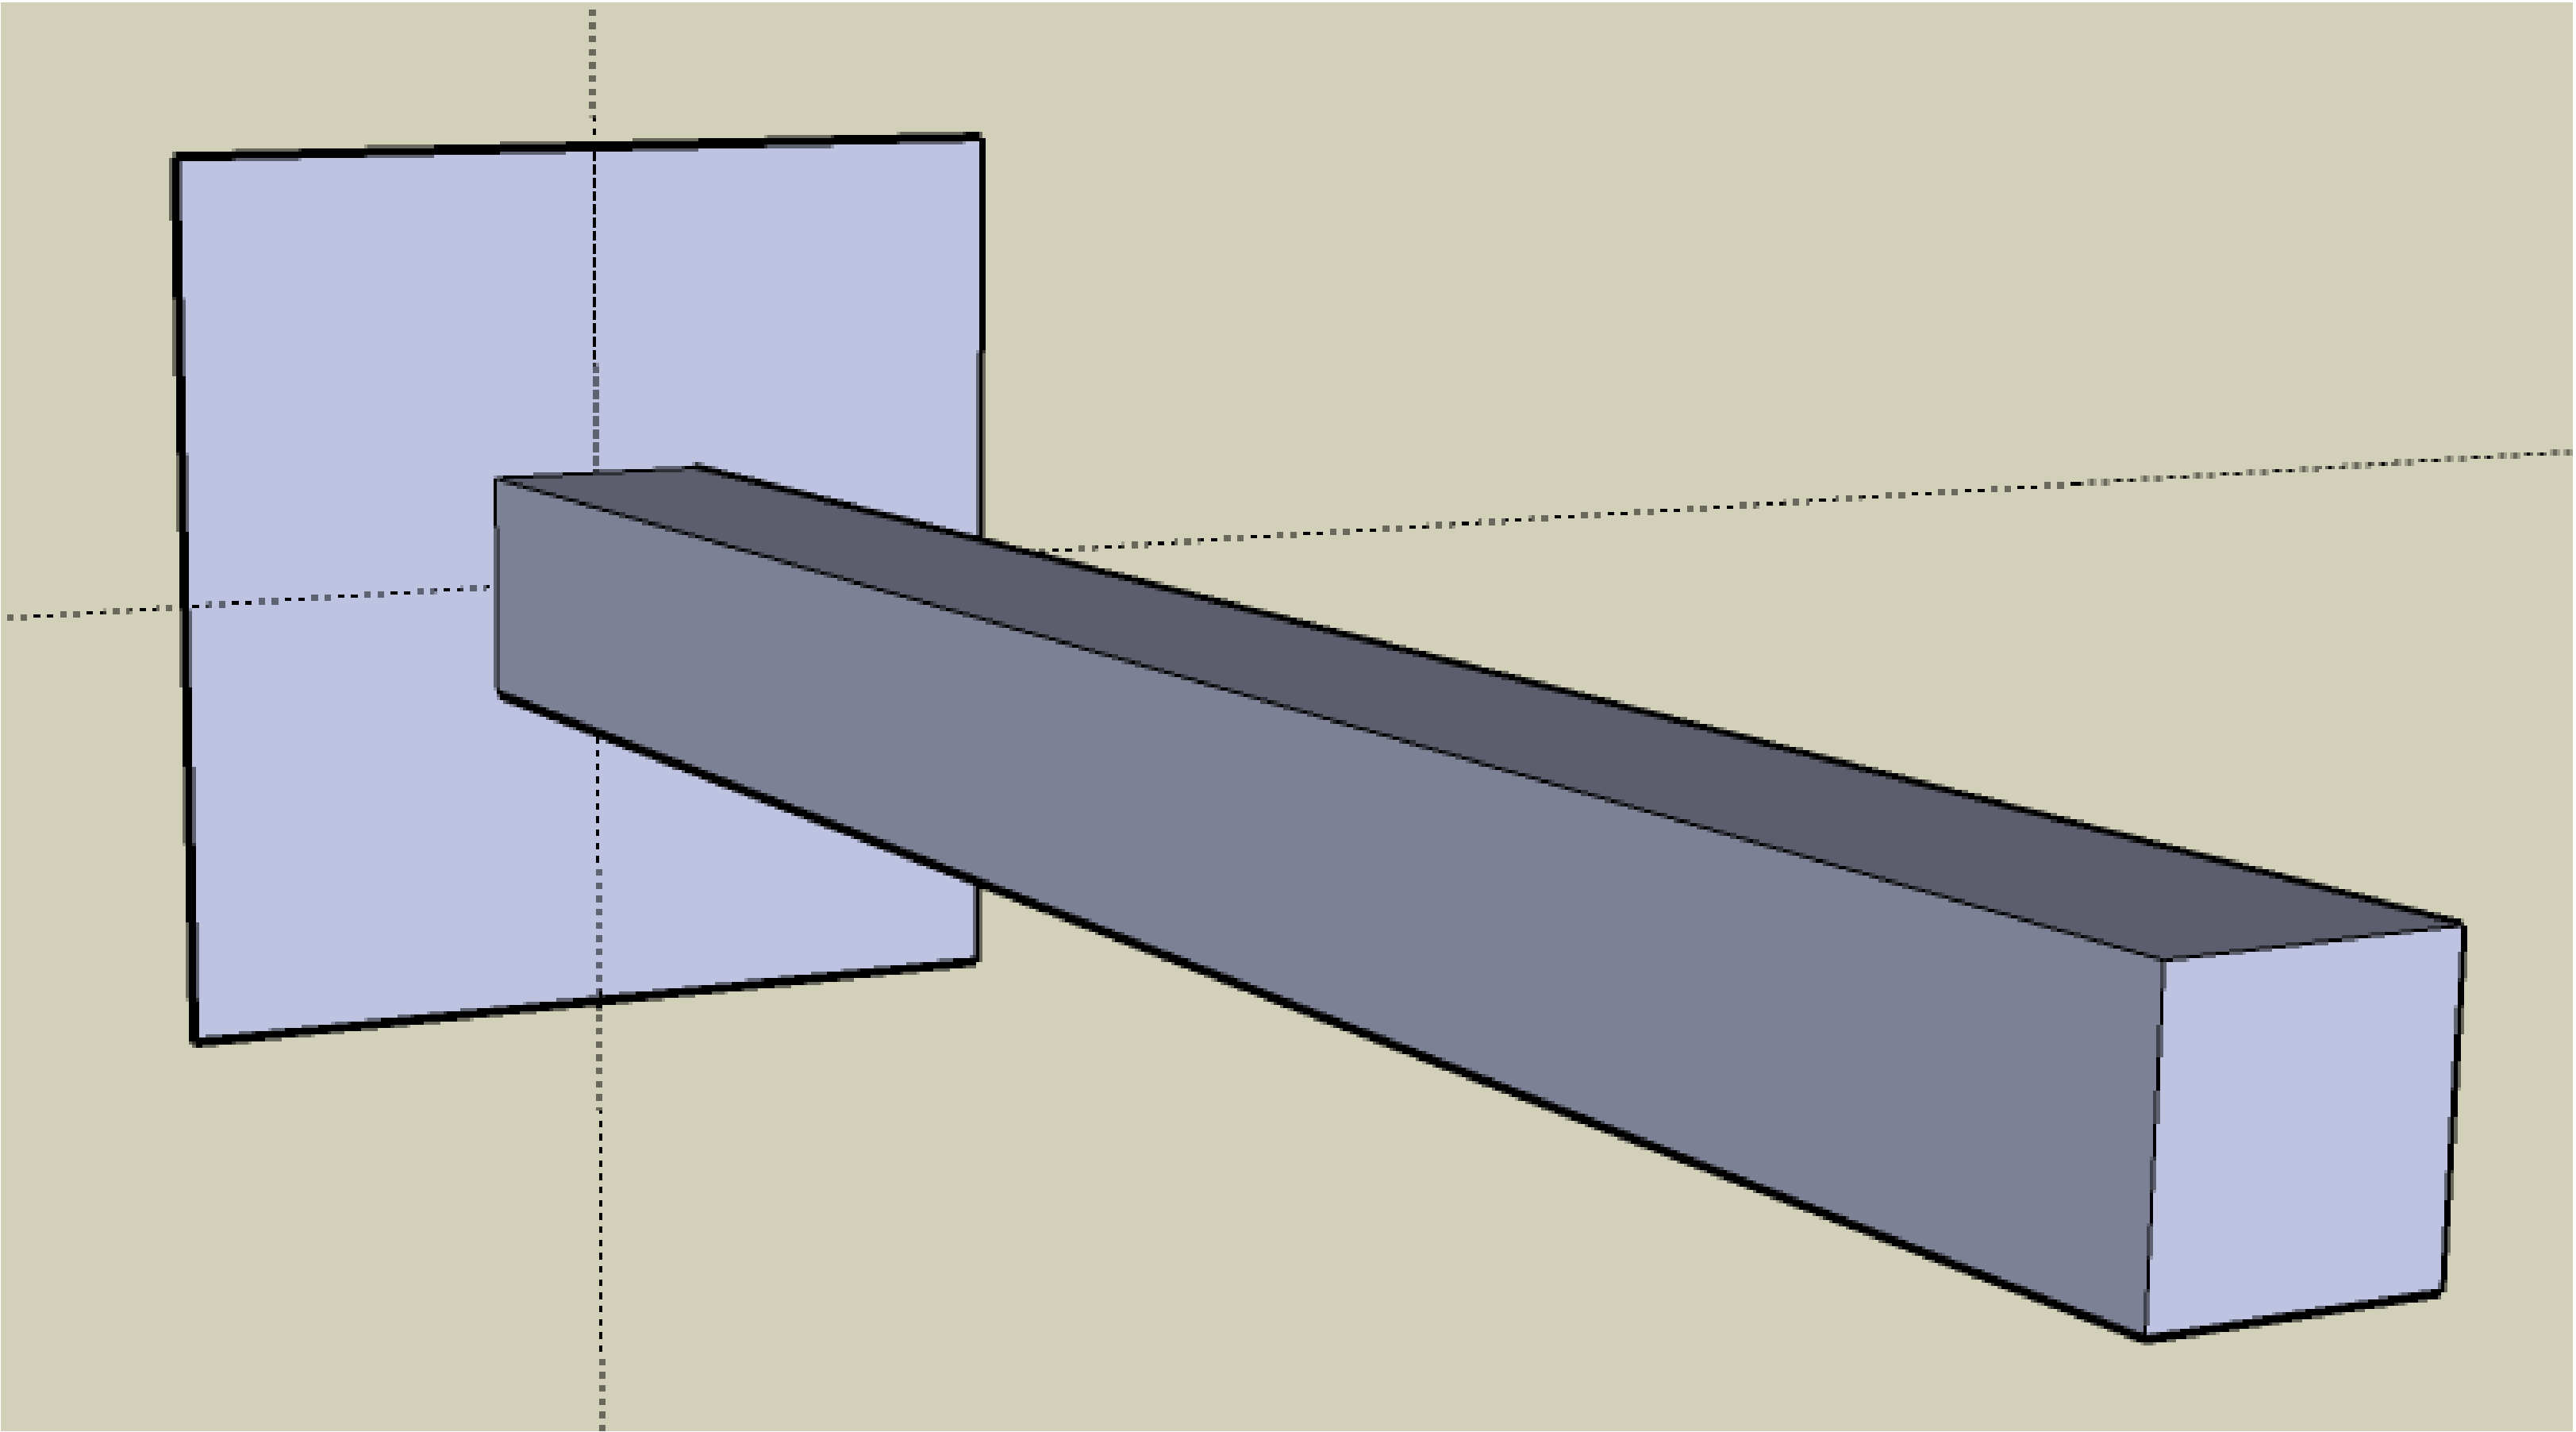
\includegraphics[width=3.5in]{graphics/notes_06_LongPin3D}
\end{center}

\vfill
\vfill

\newpage

The rate of heat flow from a metal fin to the environment will
proportional to the temperature difference between the fin, $T$, and
the environment, $T_\infty$. \\

\problem What issue is raised when trying to use this rule to compute
the rate of heat flow out of the fin we are considering?
 

\newpage
\topic{Numerical Integration - Motivation}
\subsection*{Numerical Integration - Motivation}

\problem Take a small slice of length $\Delta x$ of the fin.  What
advantage is there to looking at a small slice, rather than the whole
fin at once?
\vfill

How much heat is lost through that slice?
\begin{center}
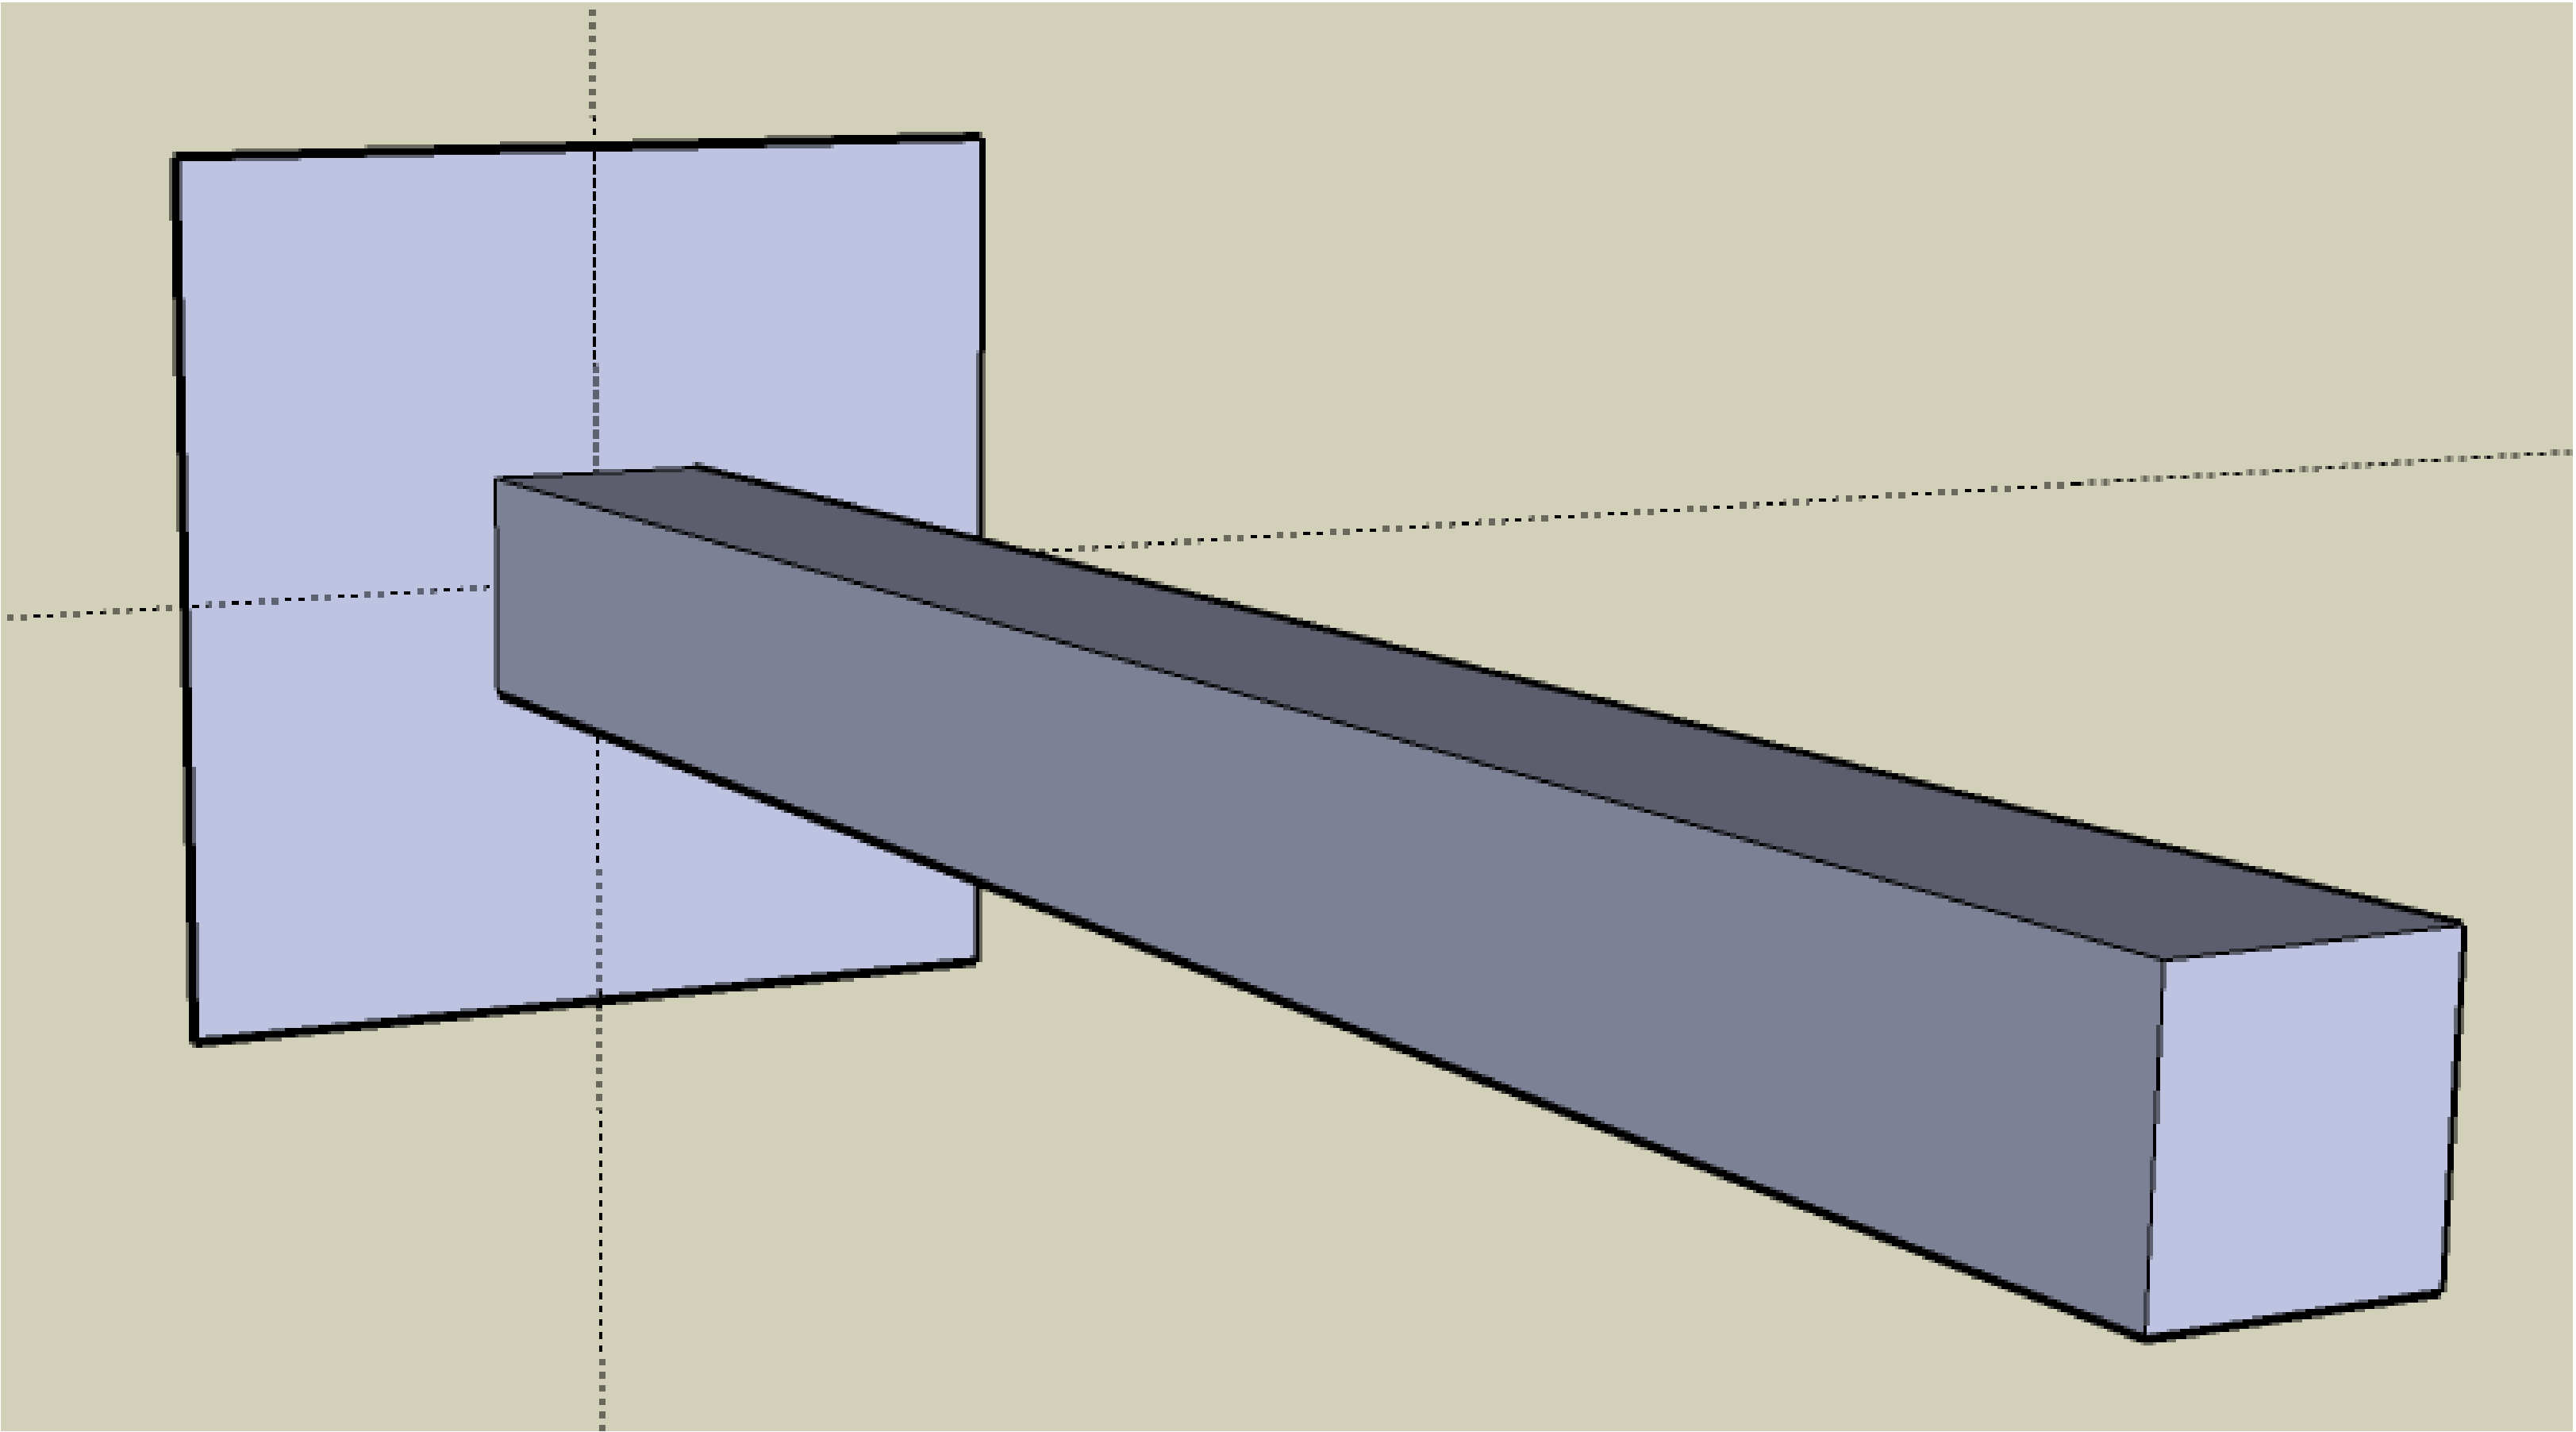
\includegraphics[width=3.5in]{graphics/notes_06_LongPin3D}
\end{center}

\vfill

Give an expression for the total amount of heat lost over
  the whole fin.

\vfill
\vfill


\newpage


\subsection*{Integration}

As soon as you see any sum of the form $\sum \ldots \Delta x$, you
should be thinking ``integral''!

For our fin example, net heat flow to environment is
%\begin{align*}
%\int_S h (T(x) - T_{\infty} )~dA 
%\end{align*}
\vfill
If, for simplicity, we assume $T_{\infty} = 0$, our target integral becomes
%\begin{align*}
%\mbox{Heat rate} = \int_S h ~T(x)~dA 
%\end{align*}
\vfill

\newpage

\subsection*{Finding the Temperature Distribution}
To evaluate the integral, we first need to find the temperature
distribution along the fin.  Without getting into all the gory
details, the temperature along the fin will be given by the formula

$$T(x) = \frac{T_b \left(\cosh(m(L-x)) + \frac{h}{mk}\right)\left(\sinh(m(L-x))\right)}{\cosh(mL) + \frac{h}{mk} \sinh(mL)}$$

\problem What are these new $\cosh(x)$ and $\sinh(x)$ functions?



\newpage
\subsection*{Graphically}
Once we have the temperature distribution, we can graph it along the
length of the fin to see if it makes sense.

\begin{center}
\begin{minipage}{4.0in}
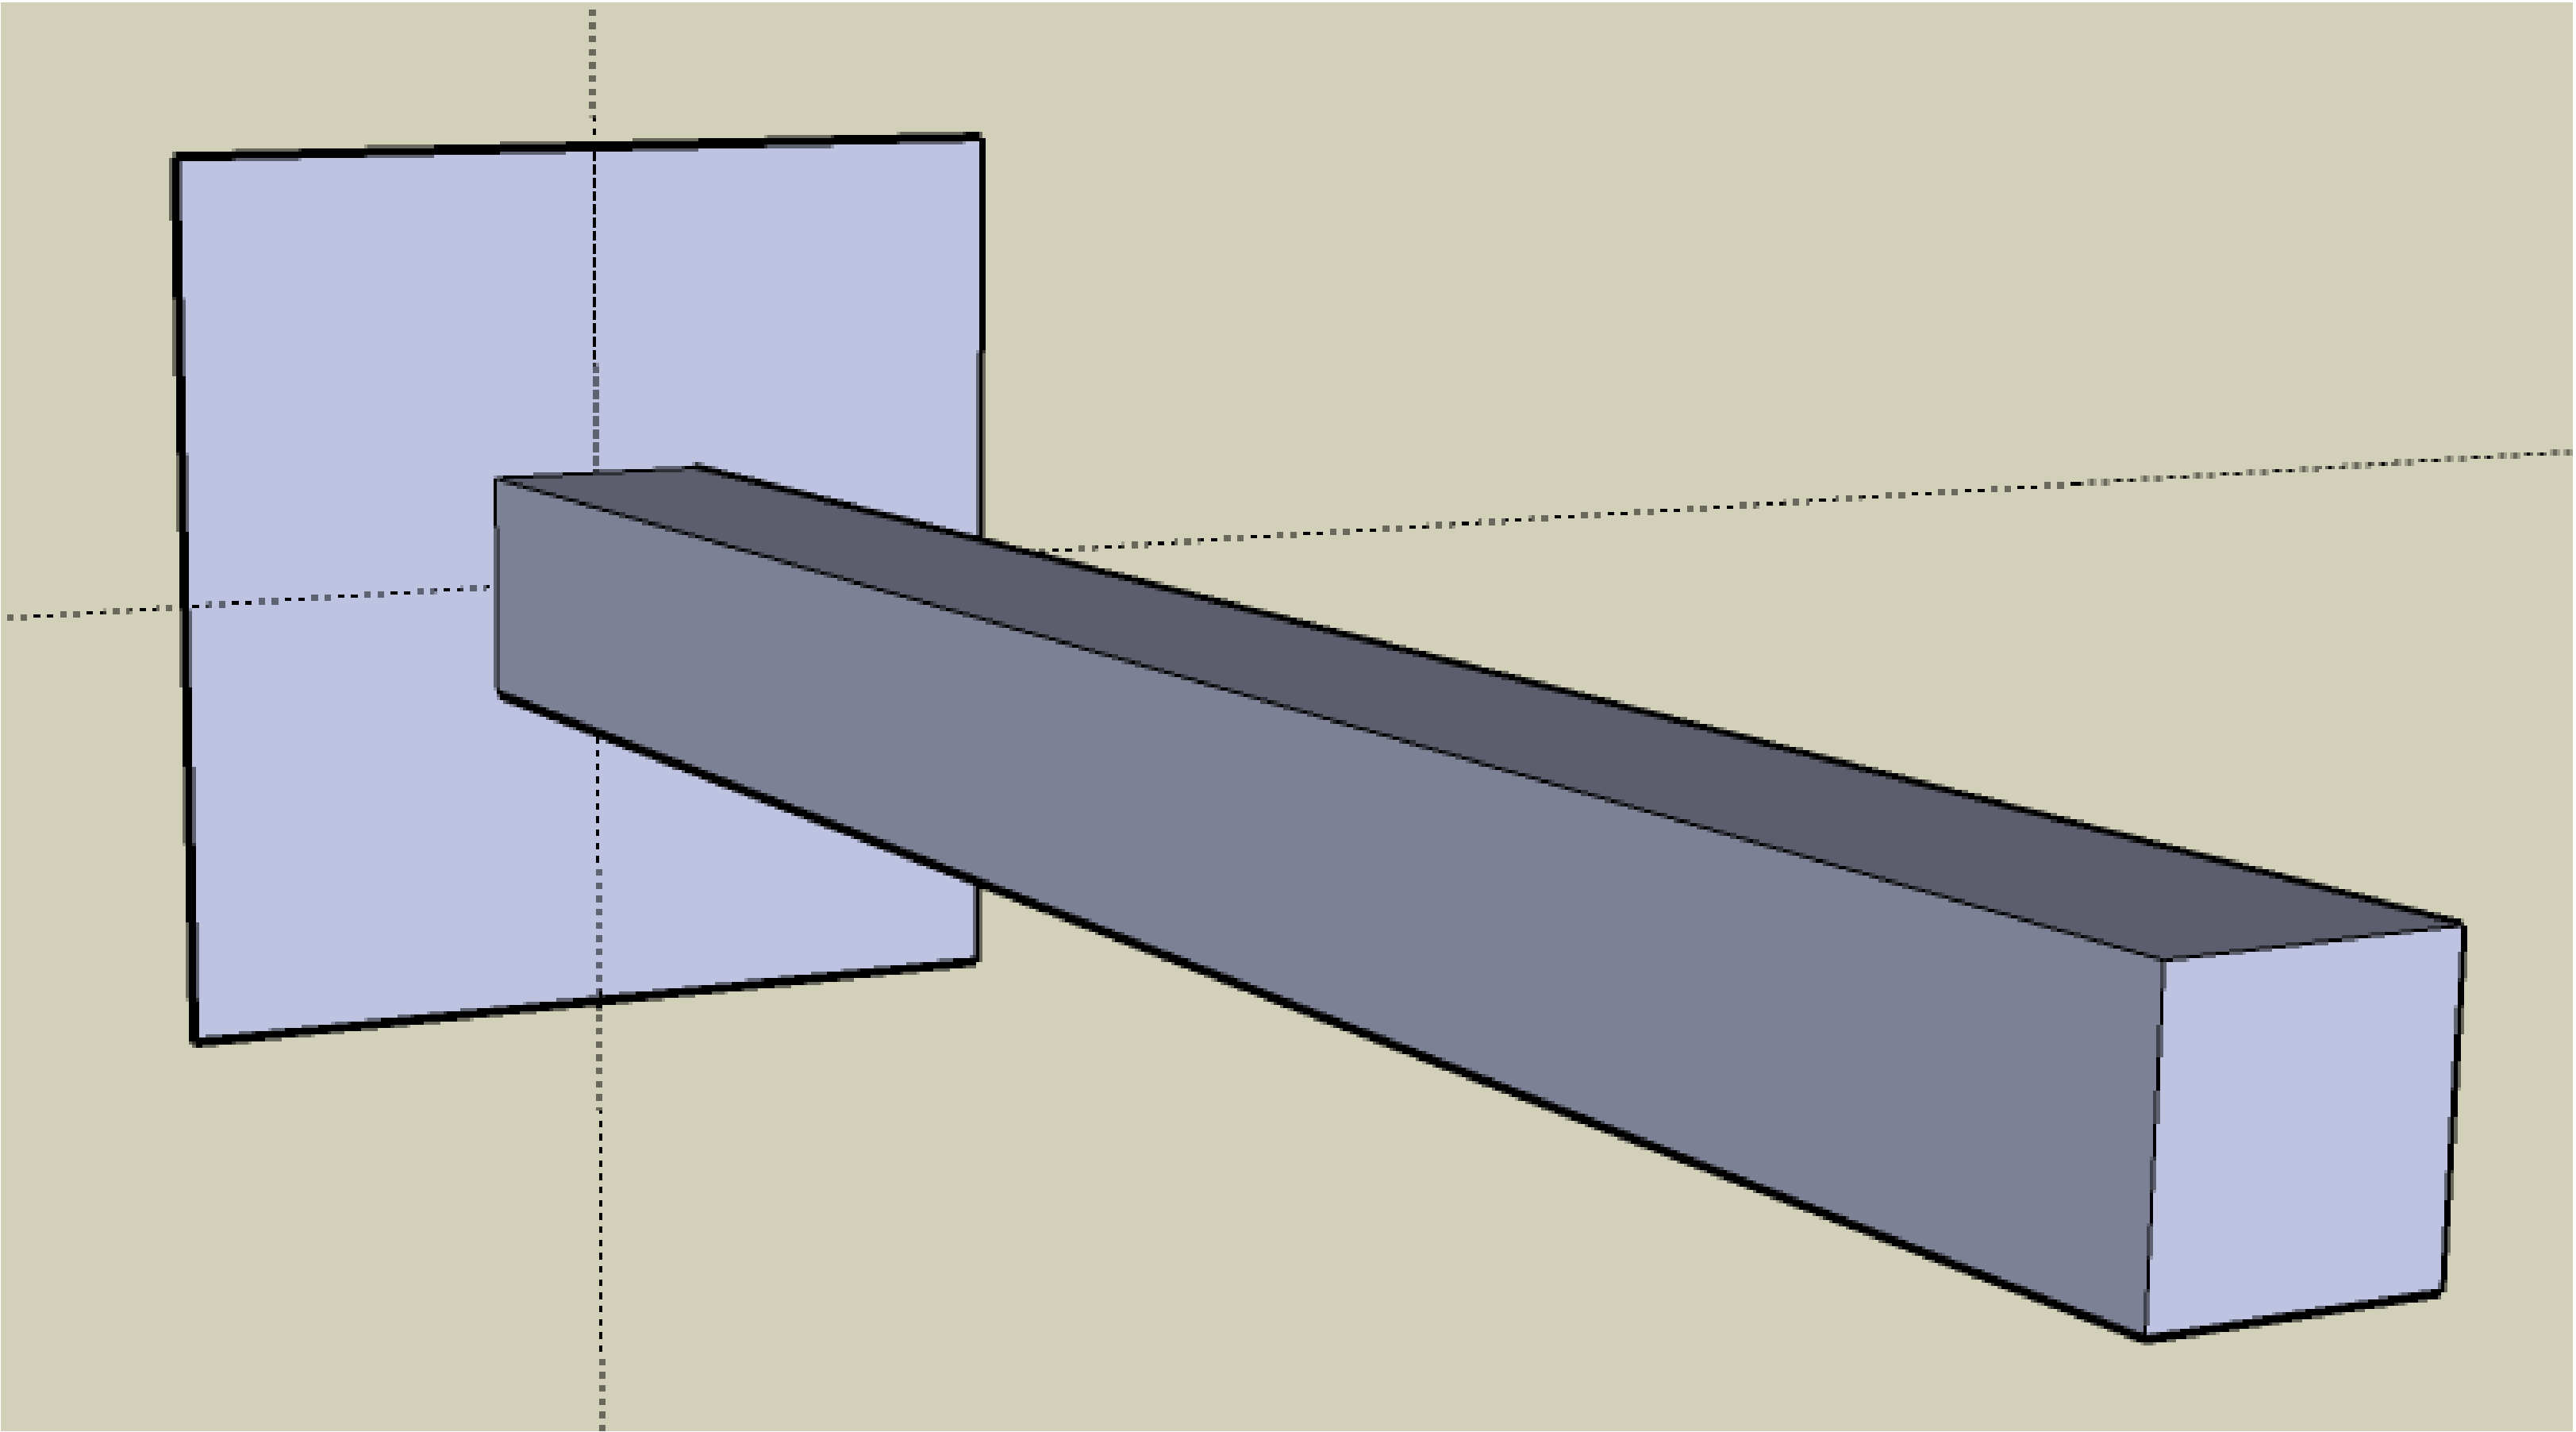
\includegraphics[width=4.0in]{graphics/notes_06_LongPin3D}
\end{minipage}
\begin{minipage}{4.0in}
\begin{center}
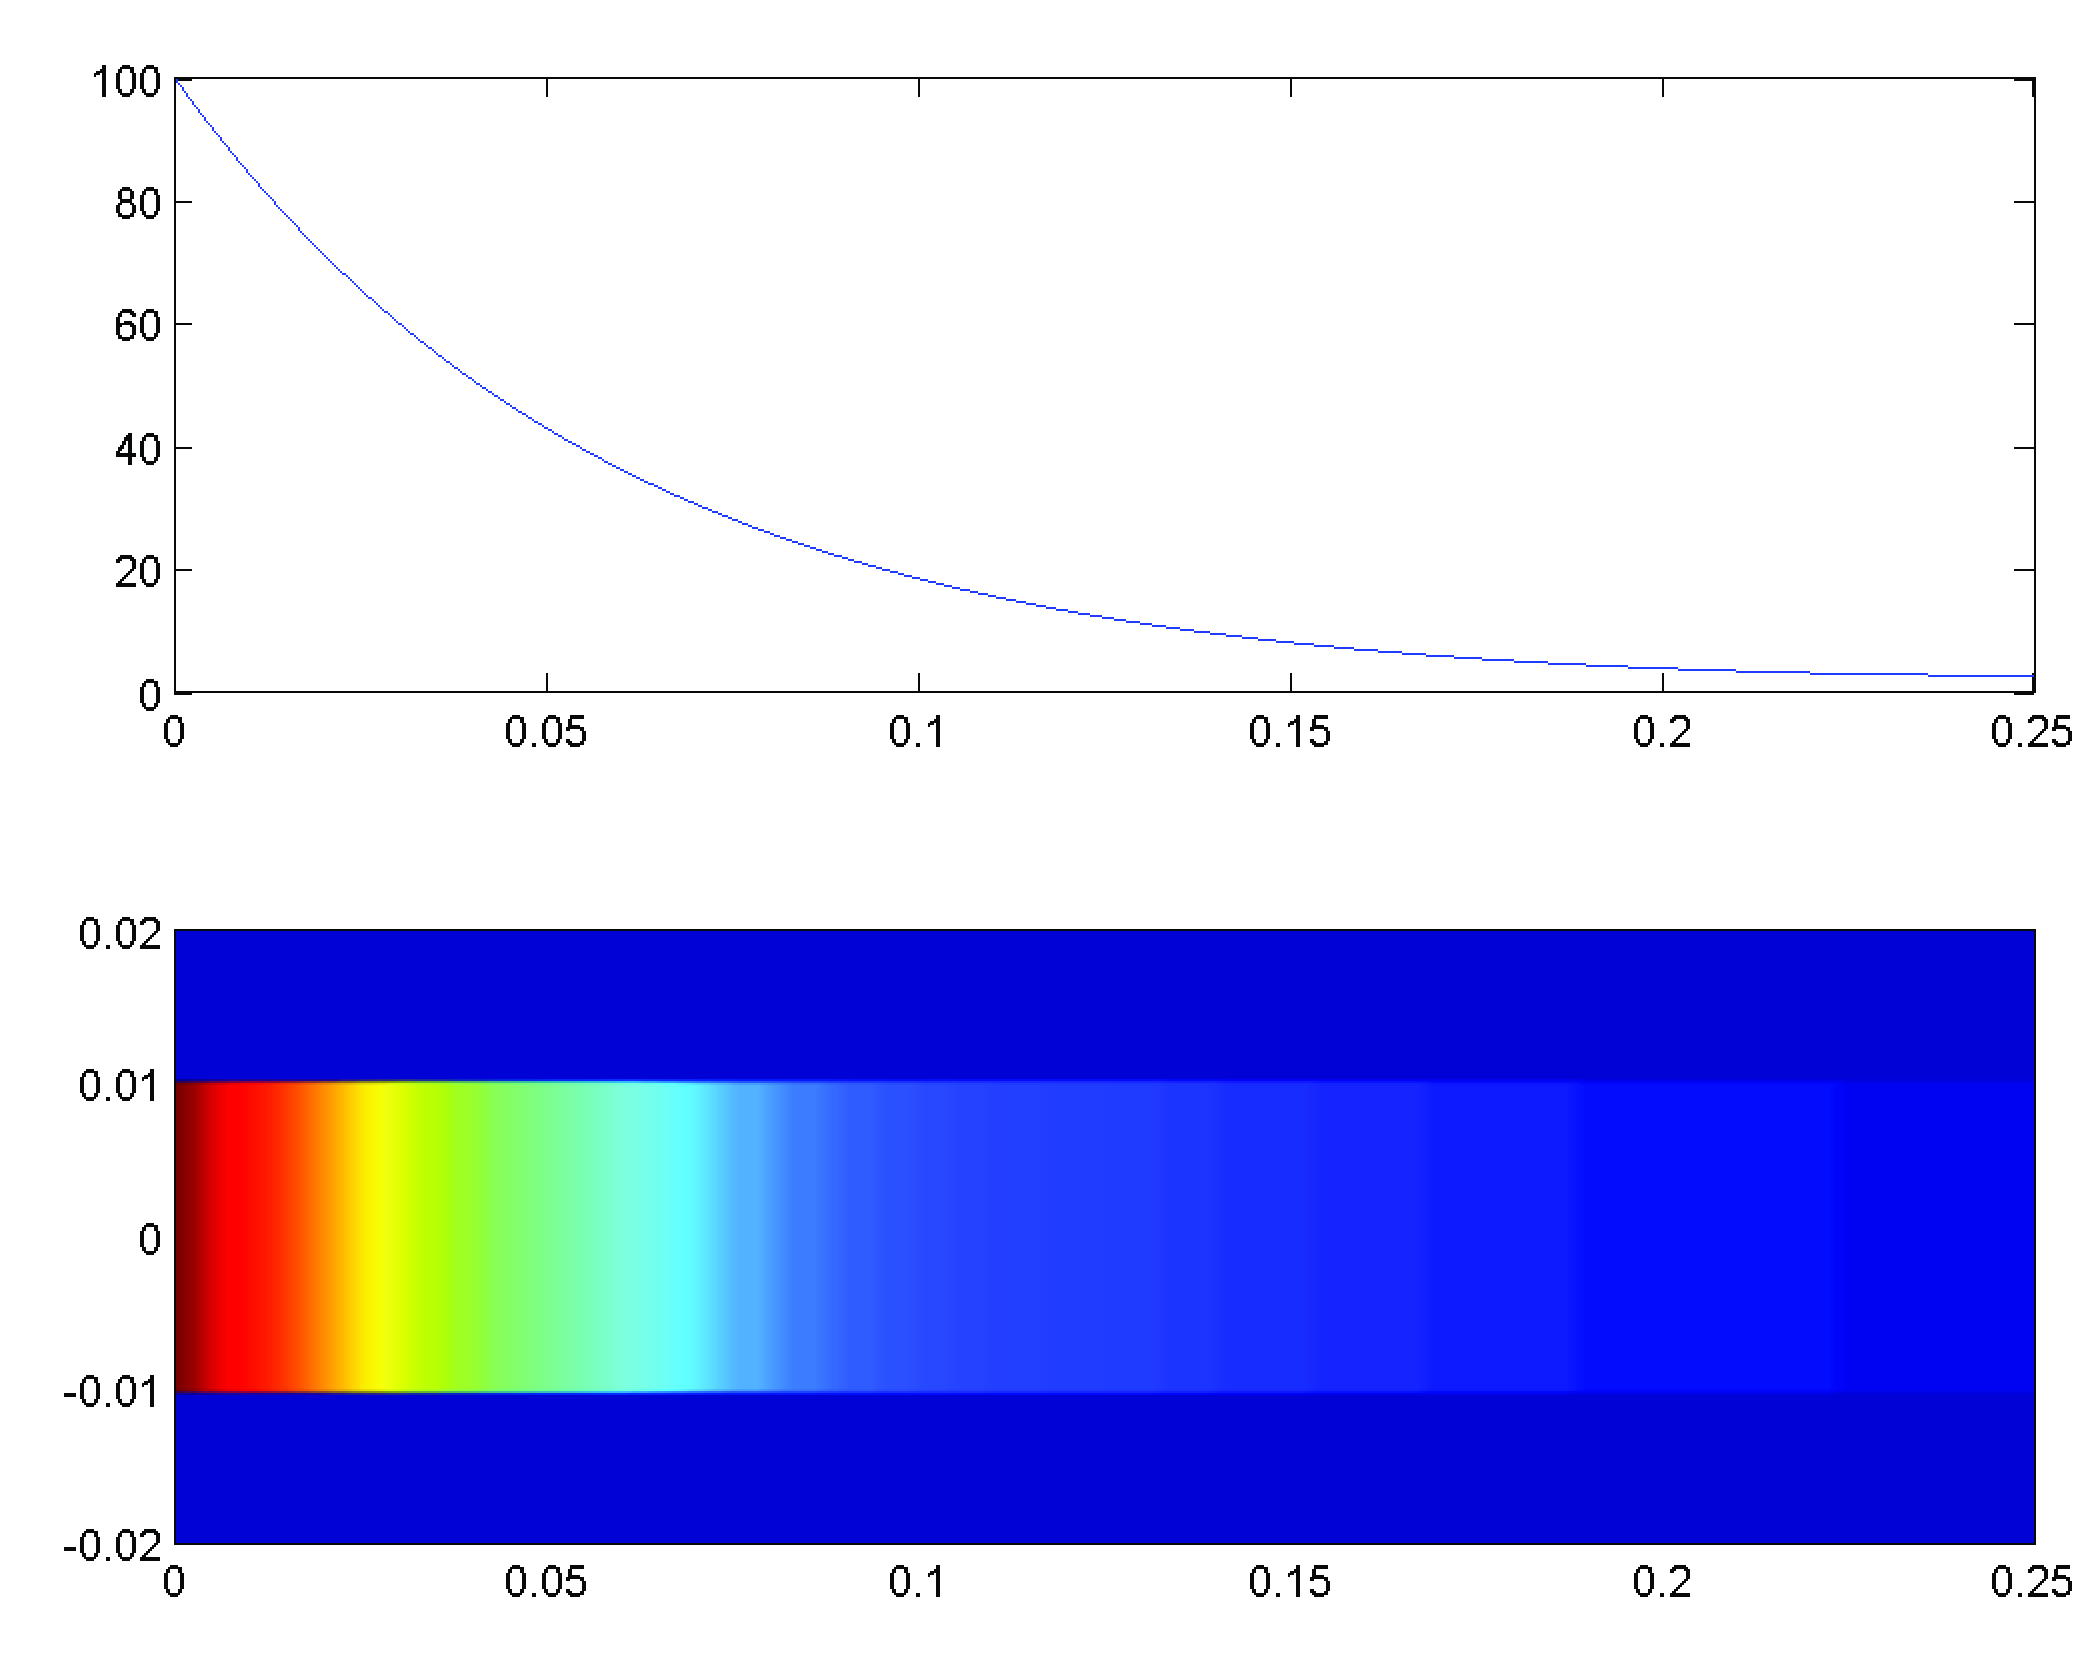
\includegraphics[height=4.0in]{graphics/notes_06_FinTemperature1}
\end{center}
\end{minipage}
\end{center}


\newpage


\topic{Computing Total Heat Loss}
\subsection*{Computing Total Heat Loss}
Now, we have addressed one challenge in our problem: we know the
steady-state temperature along the fin.  Next, we want to compute
the net rate of heat flow out, or the cooling ability of the fin.

The heat flow out of the fin is given by
$$
Q = \int_0^{L} h ~P ~T(x) ~dx   ~~~~~~~~~~ (T_\infty \mbox{ assumed = 0})
$$
Our first approach, if it is possible, should be direct
anti-differentiation (think $\int x^2 ~dx = \frac{1}{3}x^3$).

For this problem, given the earlier temperature we found, $T(x)$, we
{\bf can} evaluate the integral exactly:
$$ \large
Q =
\frac{1}{2}\frac{T_b~P~h~(m~k~exp(2~m~L)-m~k+h~exp(2~m~L)+h-2~h~exp(m~L))}{m(\cosh(m~L)~m~k+h~\sinh(m~L))~exp(-m~L)}
$$
 

Evaluated with appropriate constants for the material, base temp,
etc. we would obtain the final value $$Q = 2.363 \mbox{ J/s}$$

\newpage

\subsection*{Comments on Anti-Derivatives}

Through this last step, we reached what would be the important
engineering goal: obtaining the {\bf numerical value} for the
integral.

When we compute integrals analytically, by using anti-derivatives, we
are doing the best possible thing. 
\begin{itemize}
\item Integrals give exact values.
\item Integrals can be re-used immediately with different constants.
\end{itemize}
Unfortunately, actually computing the numerical value of an integral
using antiderivatives isn't always an option:
\begin{itemize}
\item Some functions don't have antiderivatives.  
\vspace{1cm}
\item Sometimes we don't have a function, but only data.
\vspace{1cm}
\item Sometimes we forget how to find the anti-derivative!
\vspace{1cm}
\end{itemize}

\newpage

\topic{Numerical Quadrature}
\subsection*{Numerical Quadrature}

The word {\em quadrature} comes from the Greek challenge of trying to
{\em square the circle}, or finding the {\bf area} (in square units)
of the round circle.

When you hear {\bf quadrature} think {\bf numerical integration}.

The two common scenarios where we need {\em numerical} integration will be:
\begin{itemize}
\item {\bf Formula} for $f(x)$ known, want $\ds \int_a^b f(x) dx$
\item {\bf Data} for $f(x)$ collected at $f(x_i)$, want $\ds \int_a^b f(x)
  dx$
\end{itemize}
We will study the formula case initially, because it is easier to
experiment with.  We will continue to use our temperature example,
$$
\int_0^{L} h ~P ~T(x) ~dx = 2.36269950112023 \mbox{ J/s}
$$

\newpage

Graphically, $\displaystyle \int_0^L \underbrace{h~P~T(x)}_{f(x)}~dx$
is the area shown below:
\begin{center}
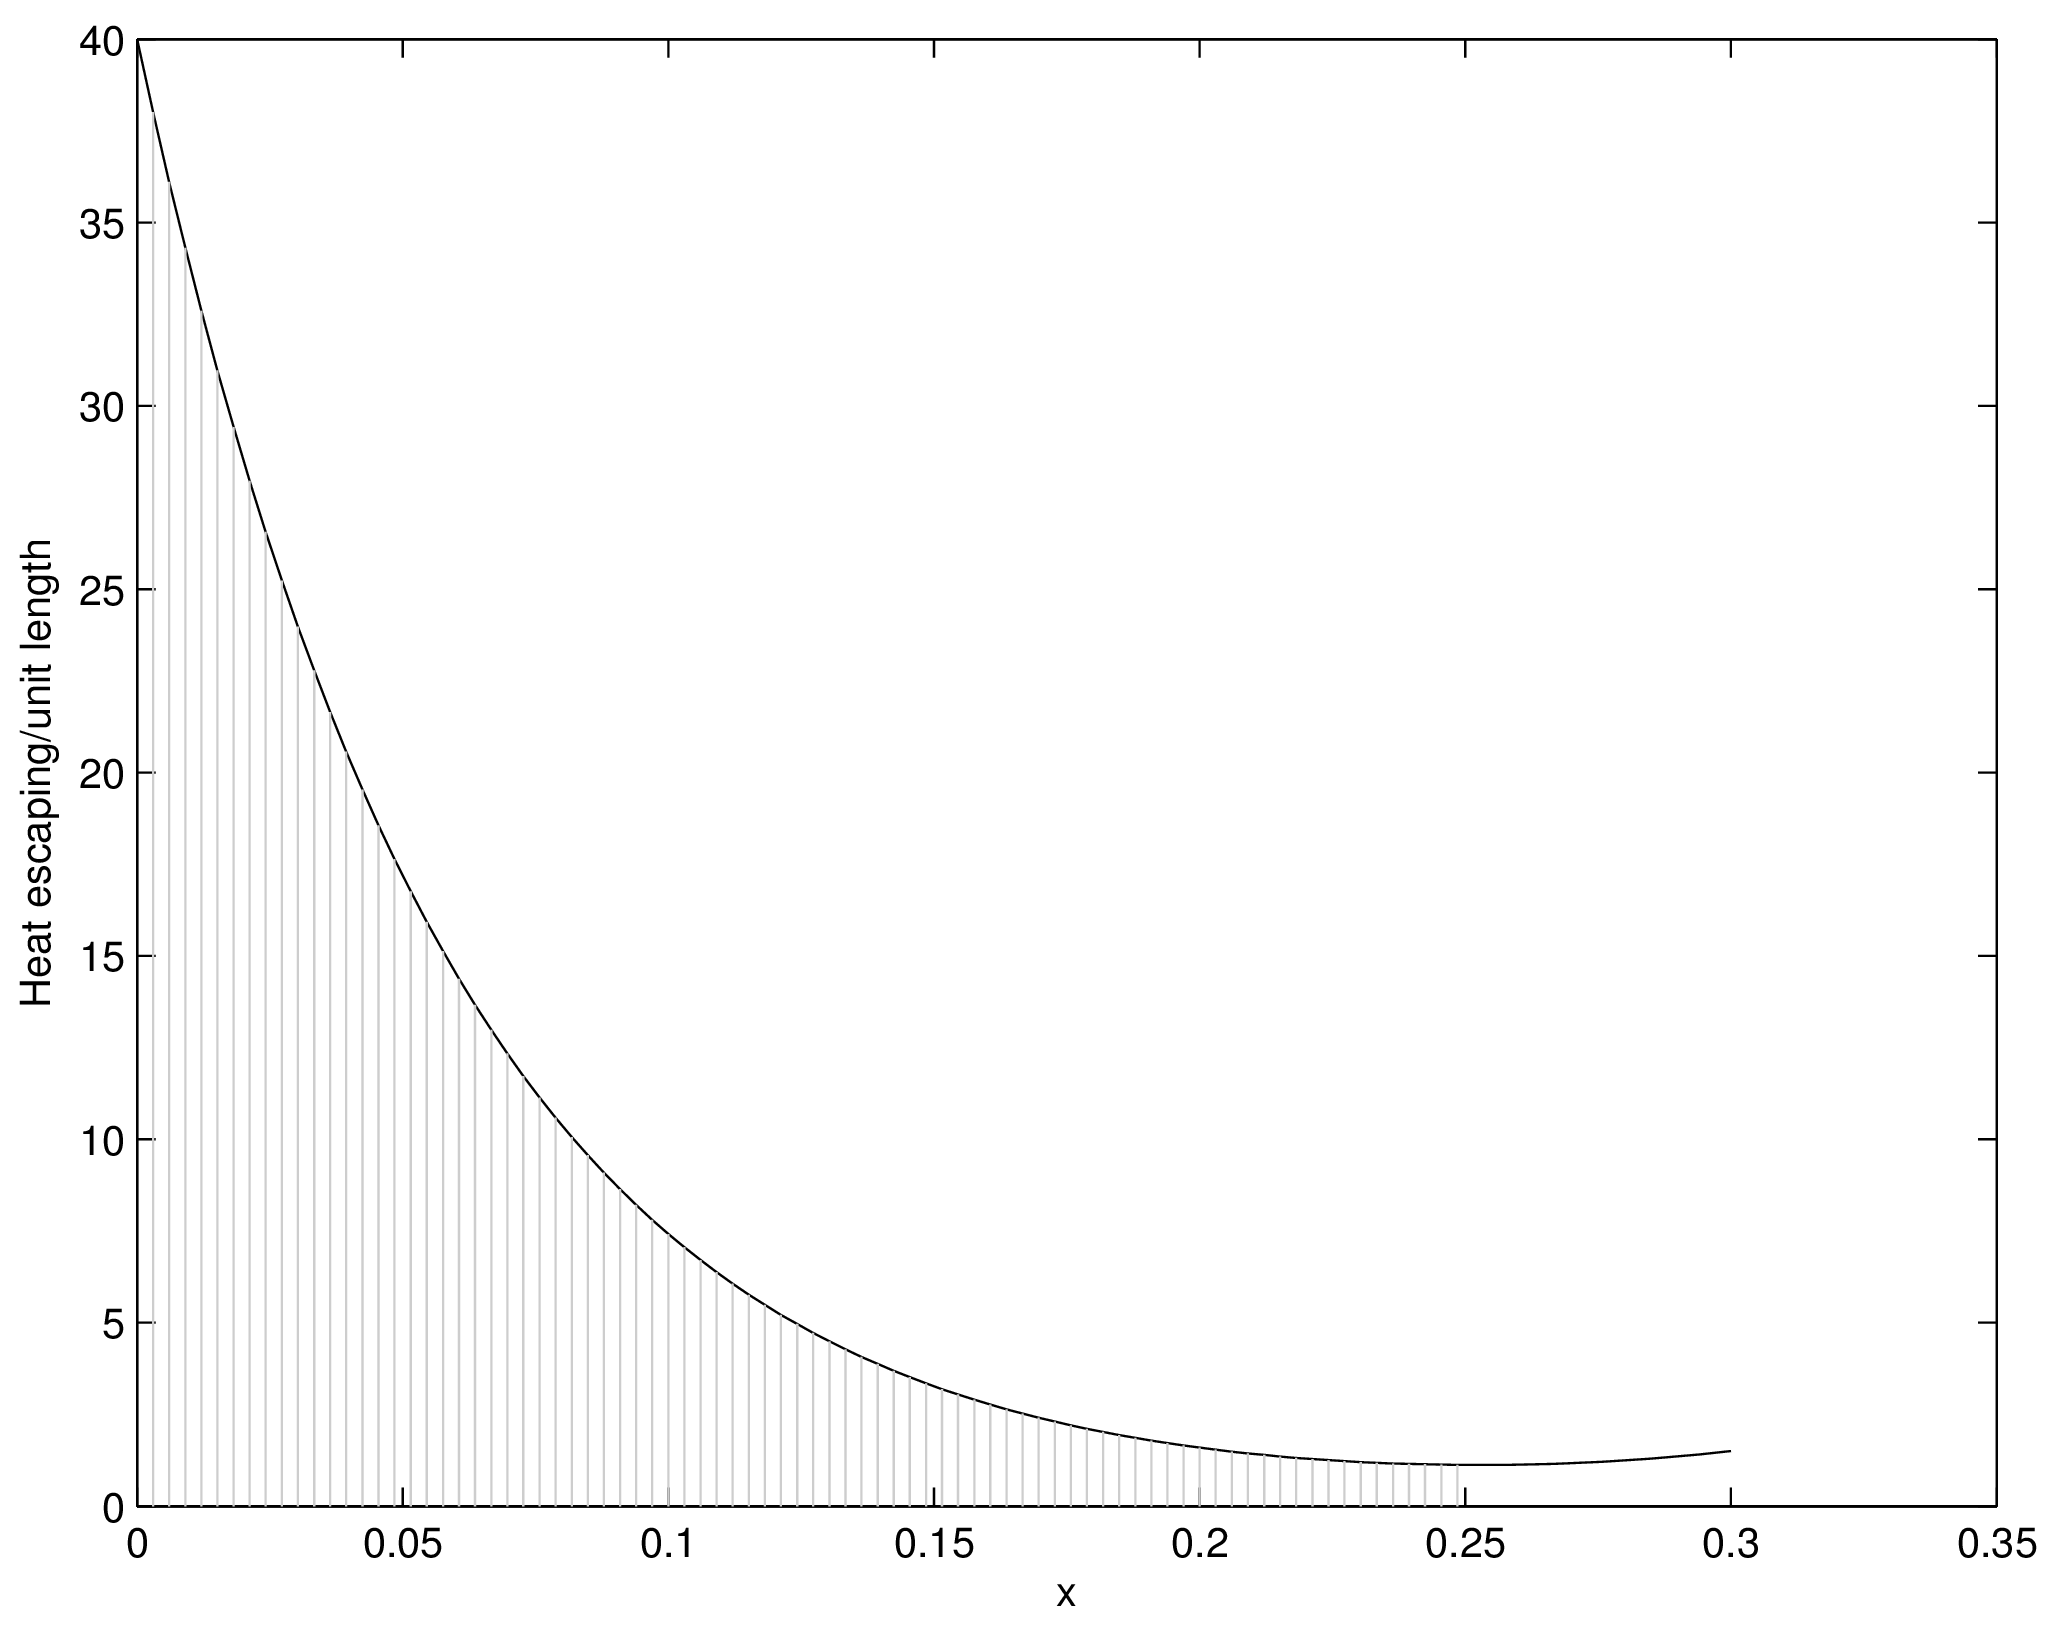
\includegraphics[height=5cm]{graphics/notes_06_f_graph_with_area}
\end{center}
Numerical integration is performed by  
\begin{itemize}
\item separating the desired interval into {\em panels}
\item on each {\em panel}, evaluating the integrand, $f(x)$ one or
  more times and those values are combined in some way to {\em estimate}
  the area of the panel
\end{itemize}

\newpage

\subsection*{Left-Hand Sum}
The simplest quadrature rule is one we have already seen: the LEFT($n$) sum.
\begin{itemize}
\item Divide the interval into $n$ panels, width $\Delta x = (b-a) / n$
\item Evaluate function at the left end point,
  $f(x_{i-1})$ on each panel. 
\item Compute the area of rectangles, $\ds \sum_{i=1}^N f(x_{i-1}) \cdot \Delta x$ or
\end{itemize}
\begin{center}
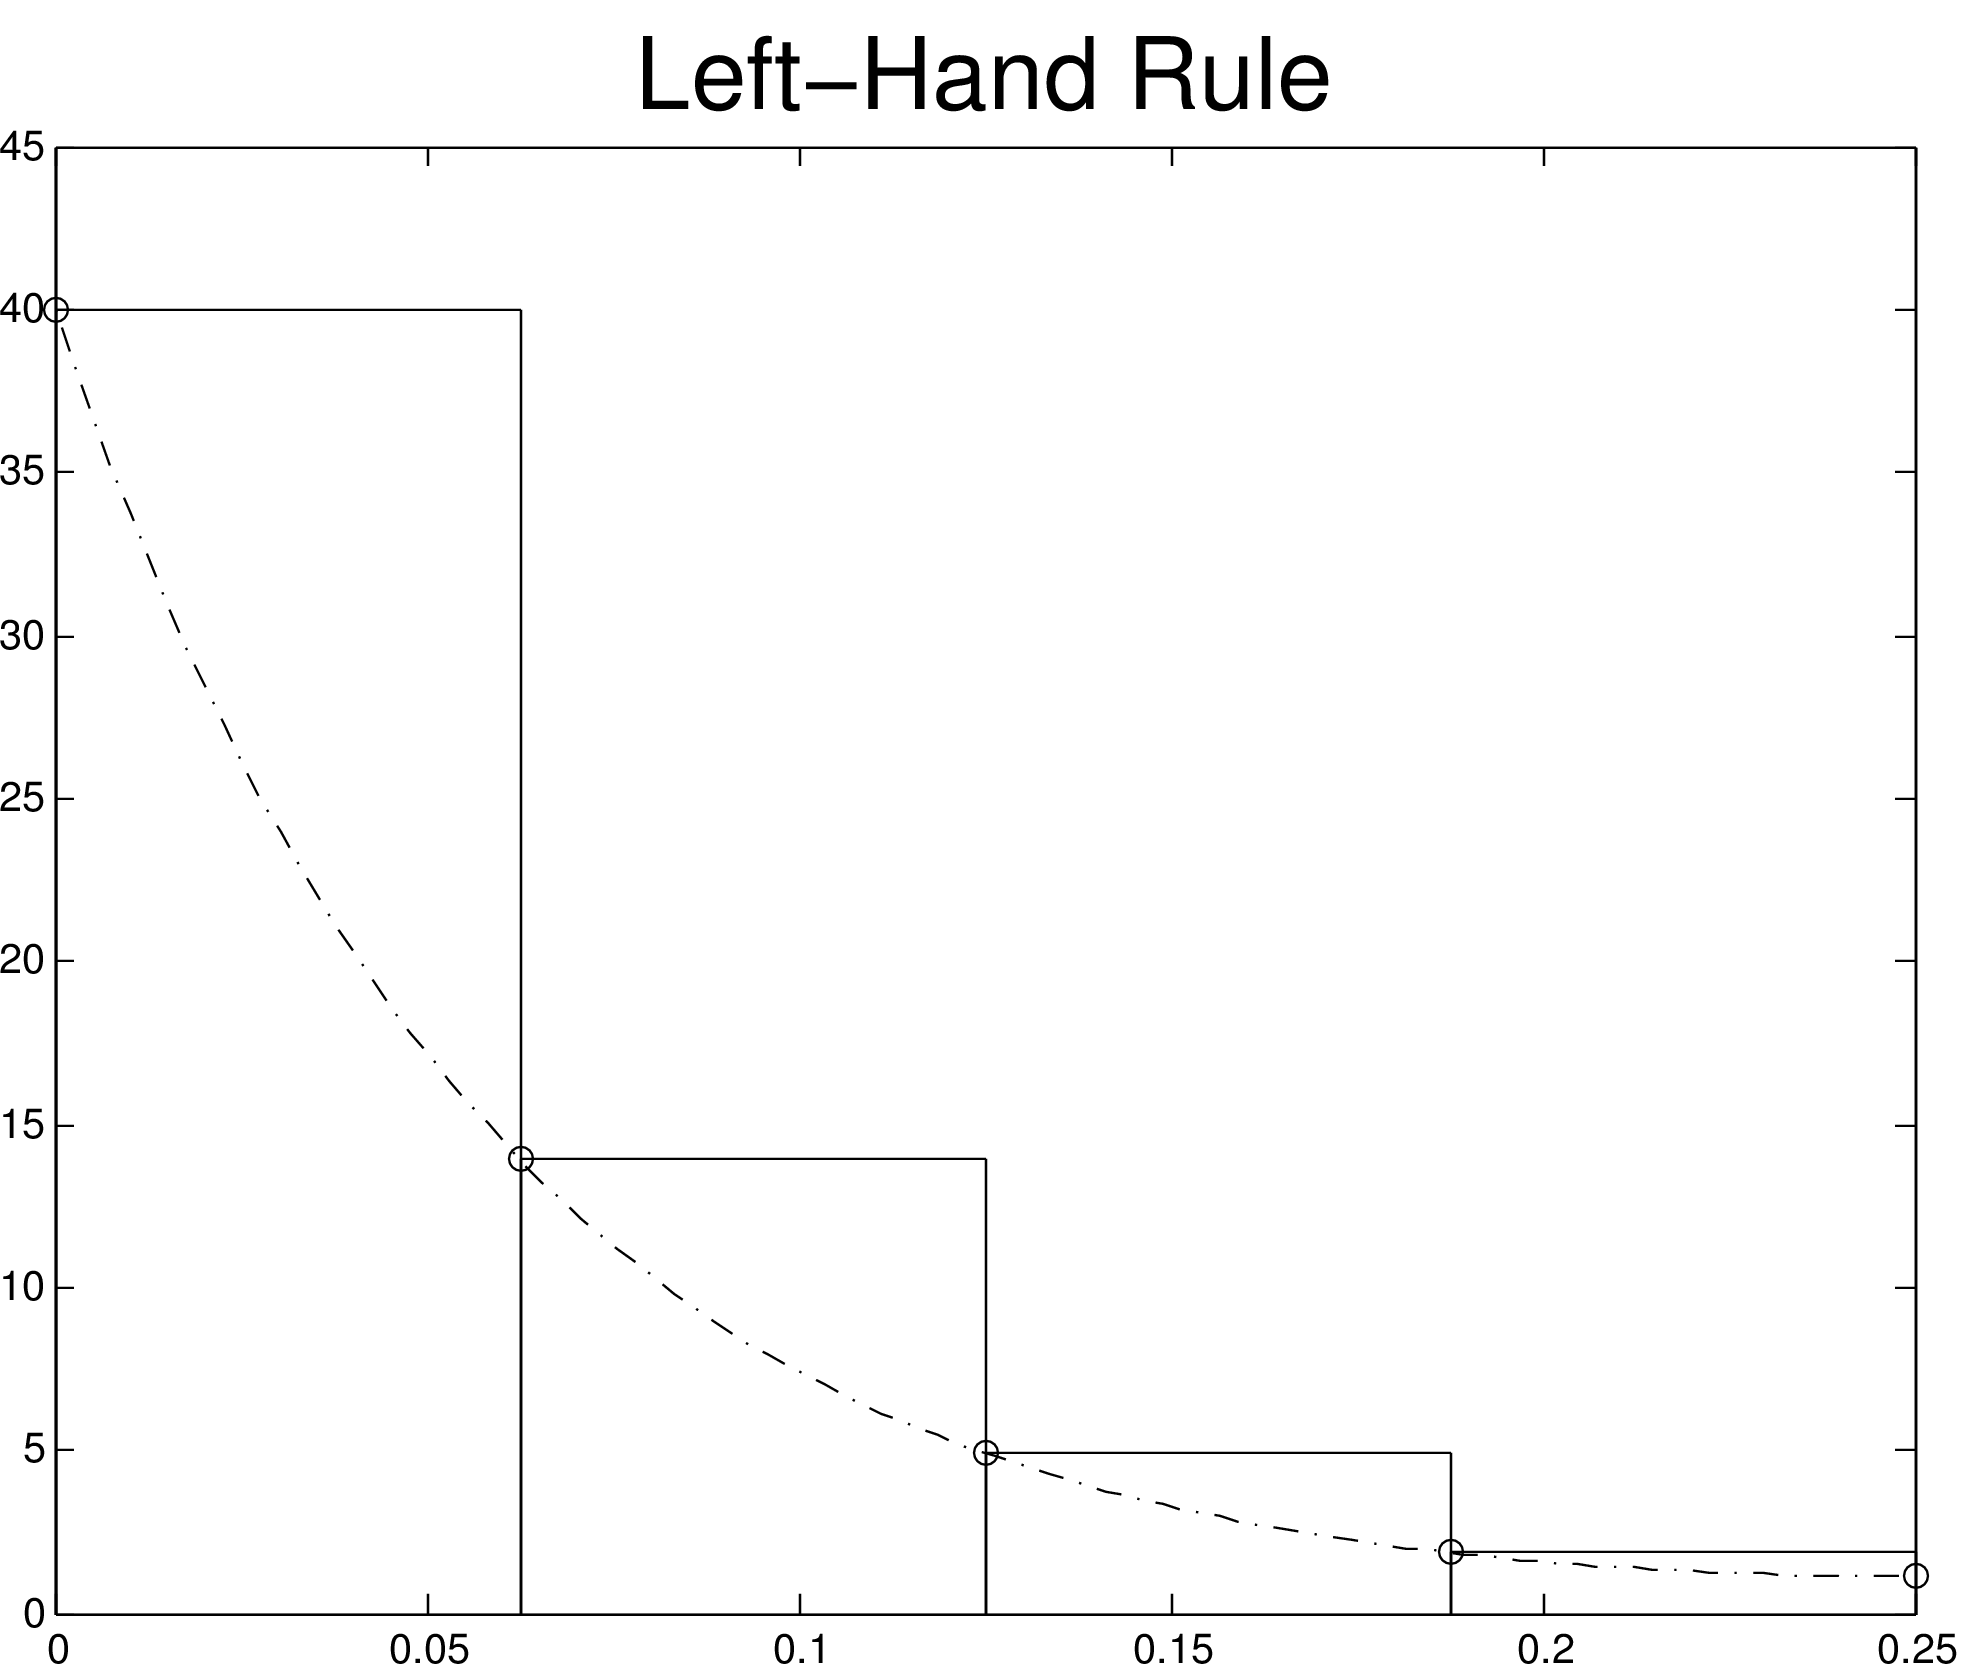
\includegraphics[height=7cm]{graphics/notes_06_f_left_hand_rule}
\end{center}

\newpage

\subsection*{Quadrature Principles}
We are approximating a complex shape with simpler shapes for which we
can compute the area. The {\bf more panels} we use, the {\bf more
  accurate} the area estimate will be:
\begin{center}
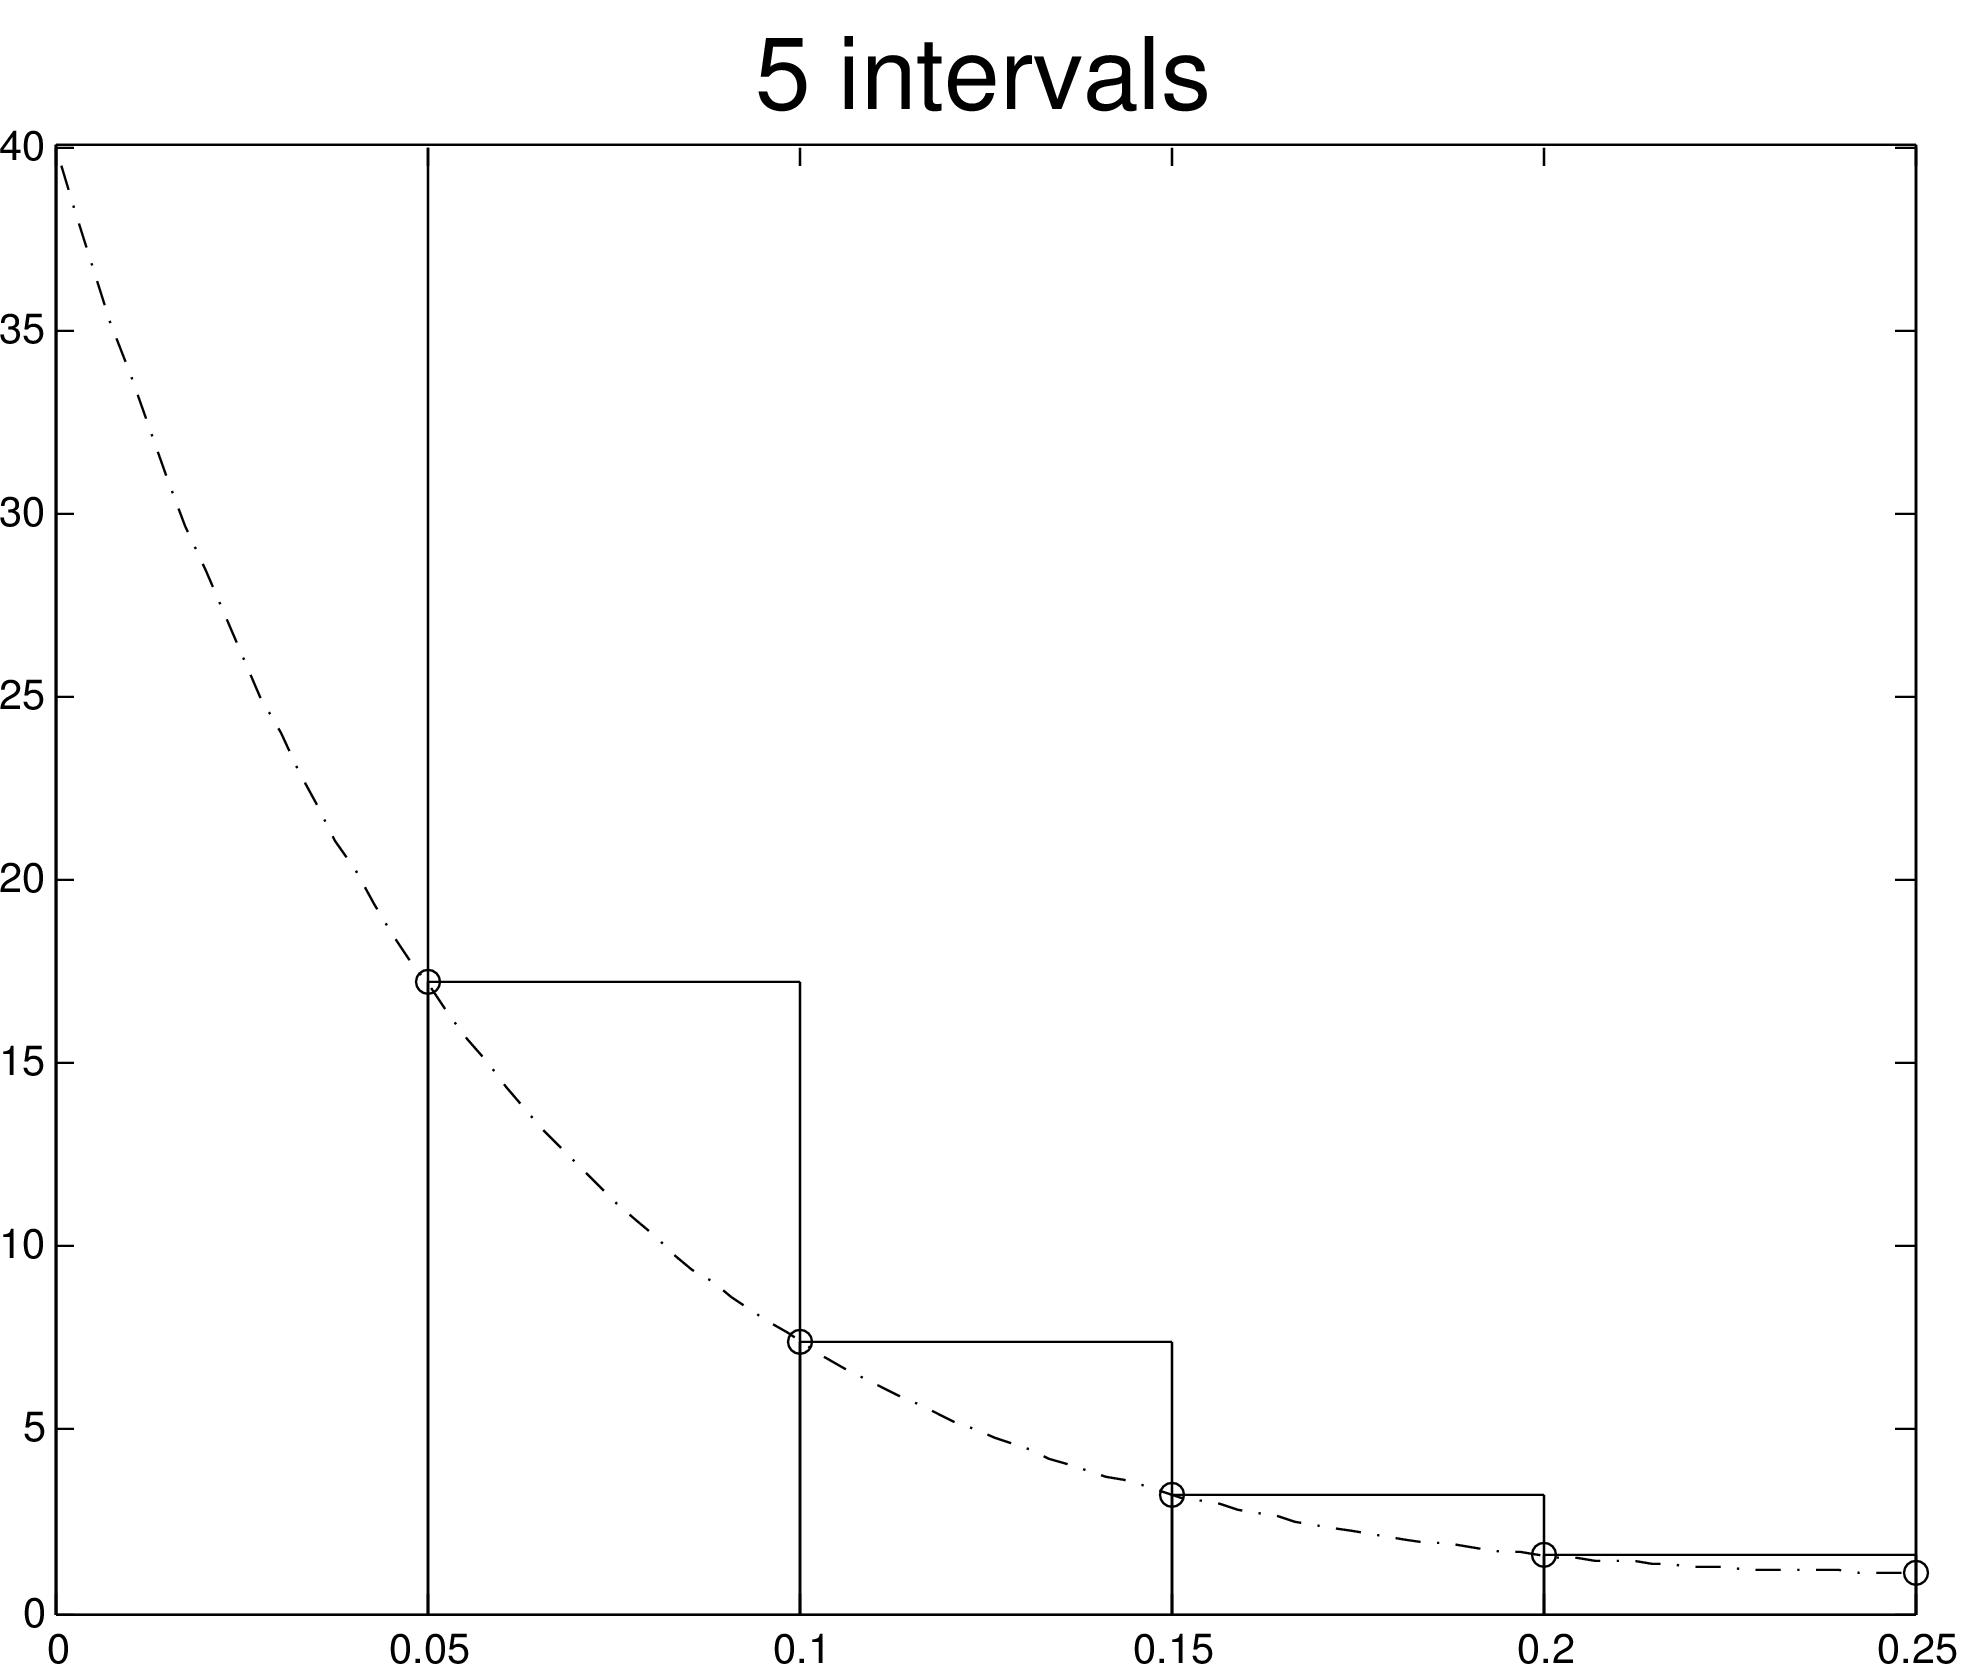
\includegraphics[height=6cm]{graphics/notes_06_f_lhr_5_intervals}
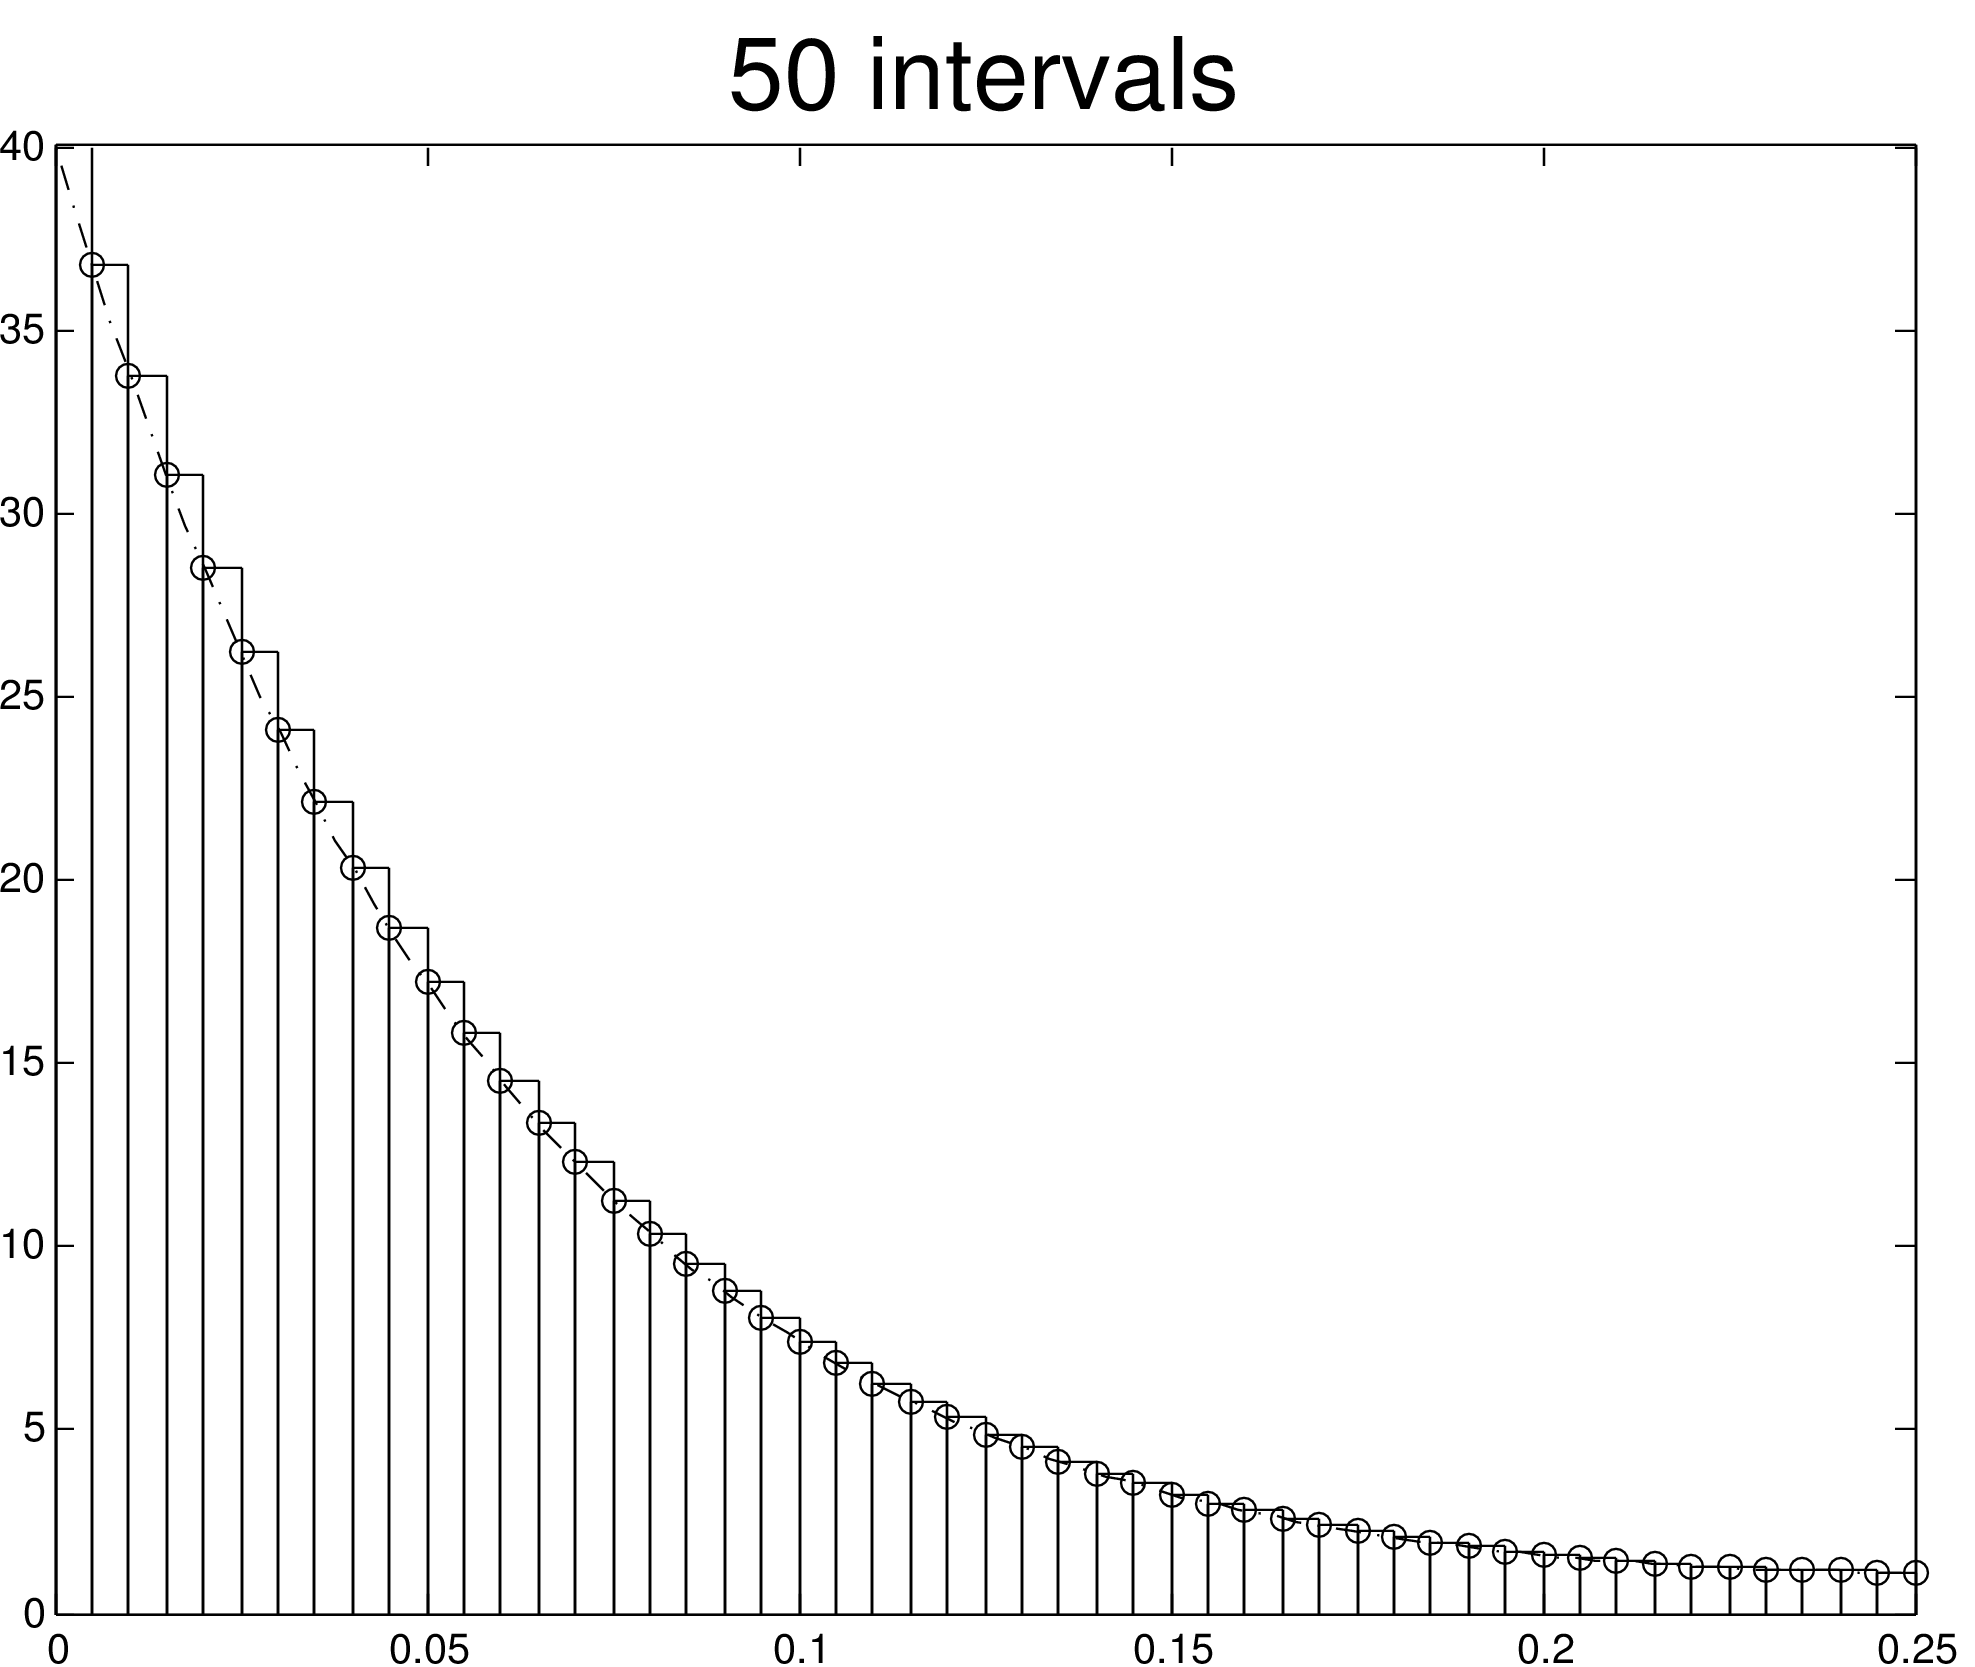
\includegraphics[height=6cm]{graphics/notes_06_f_lhr_50_intervals}
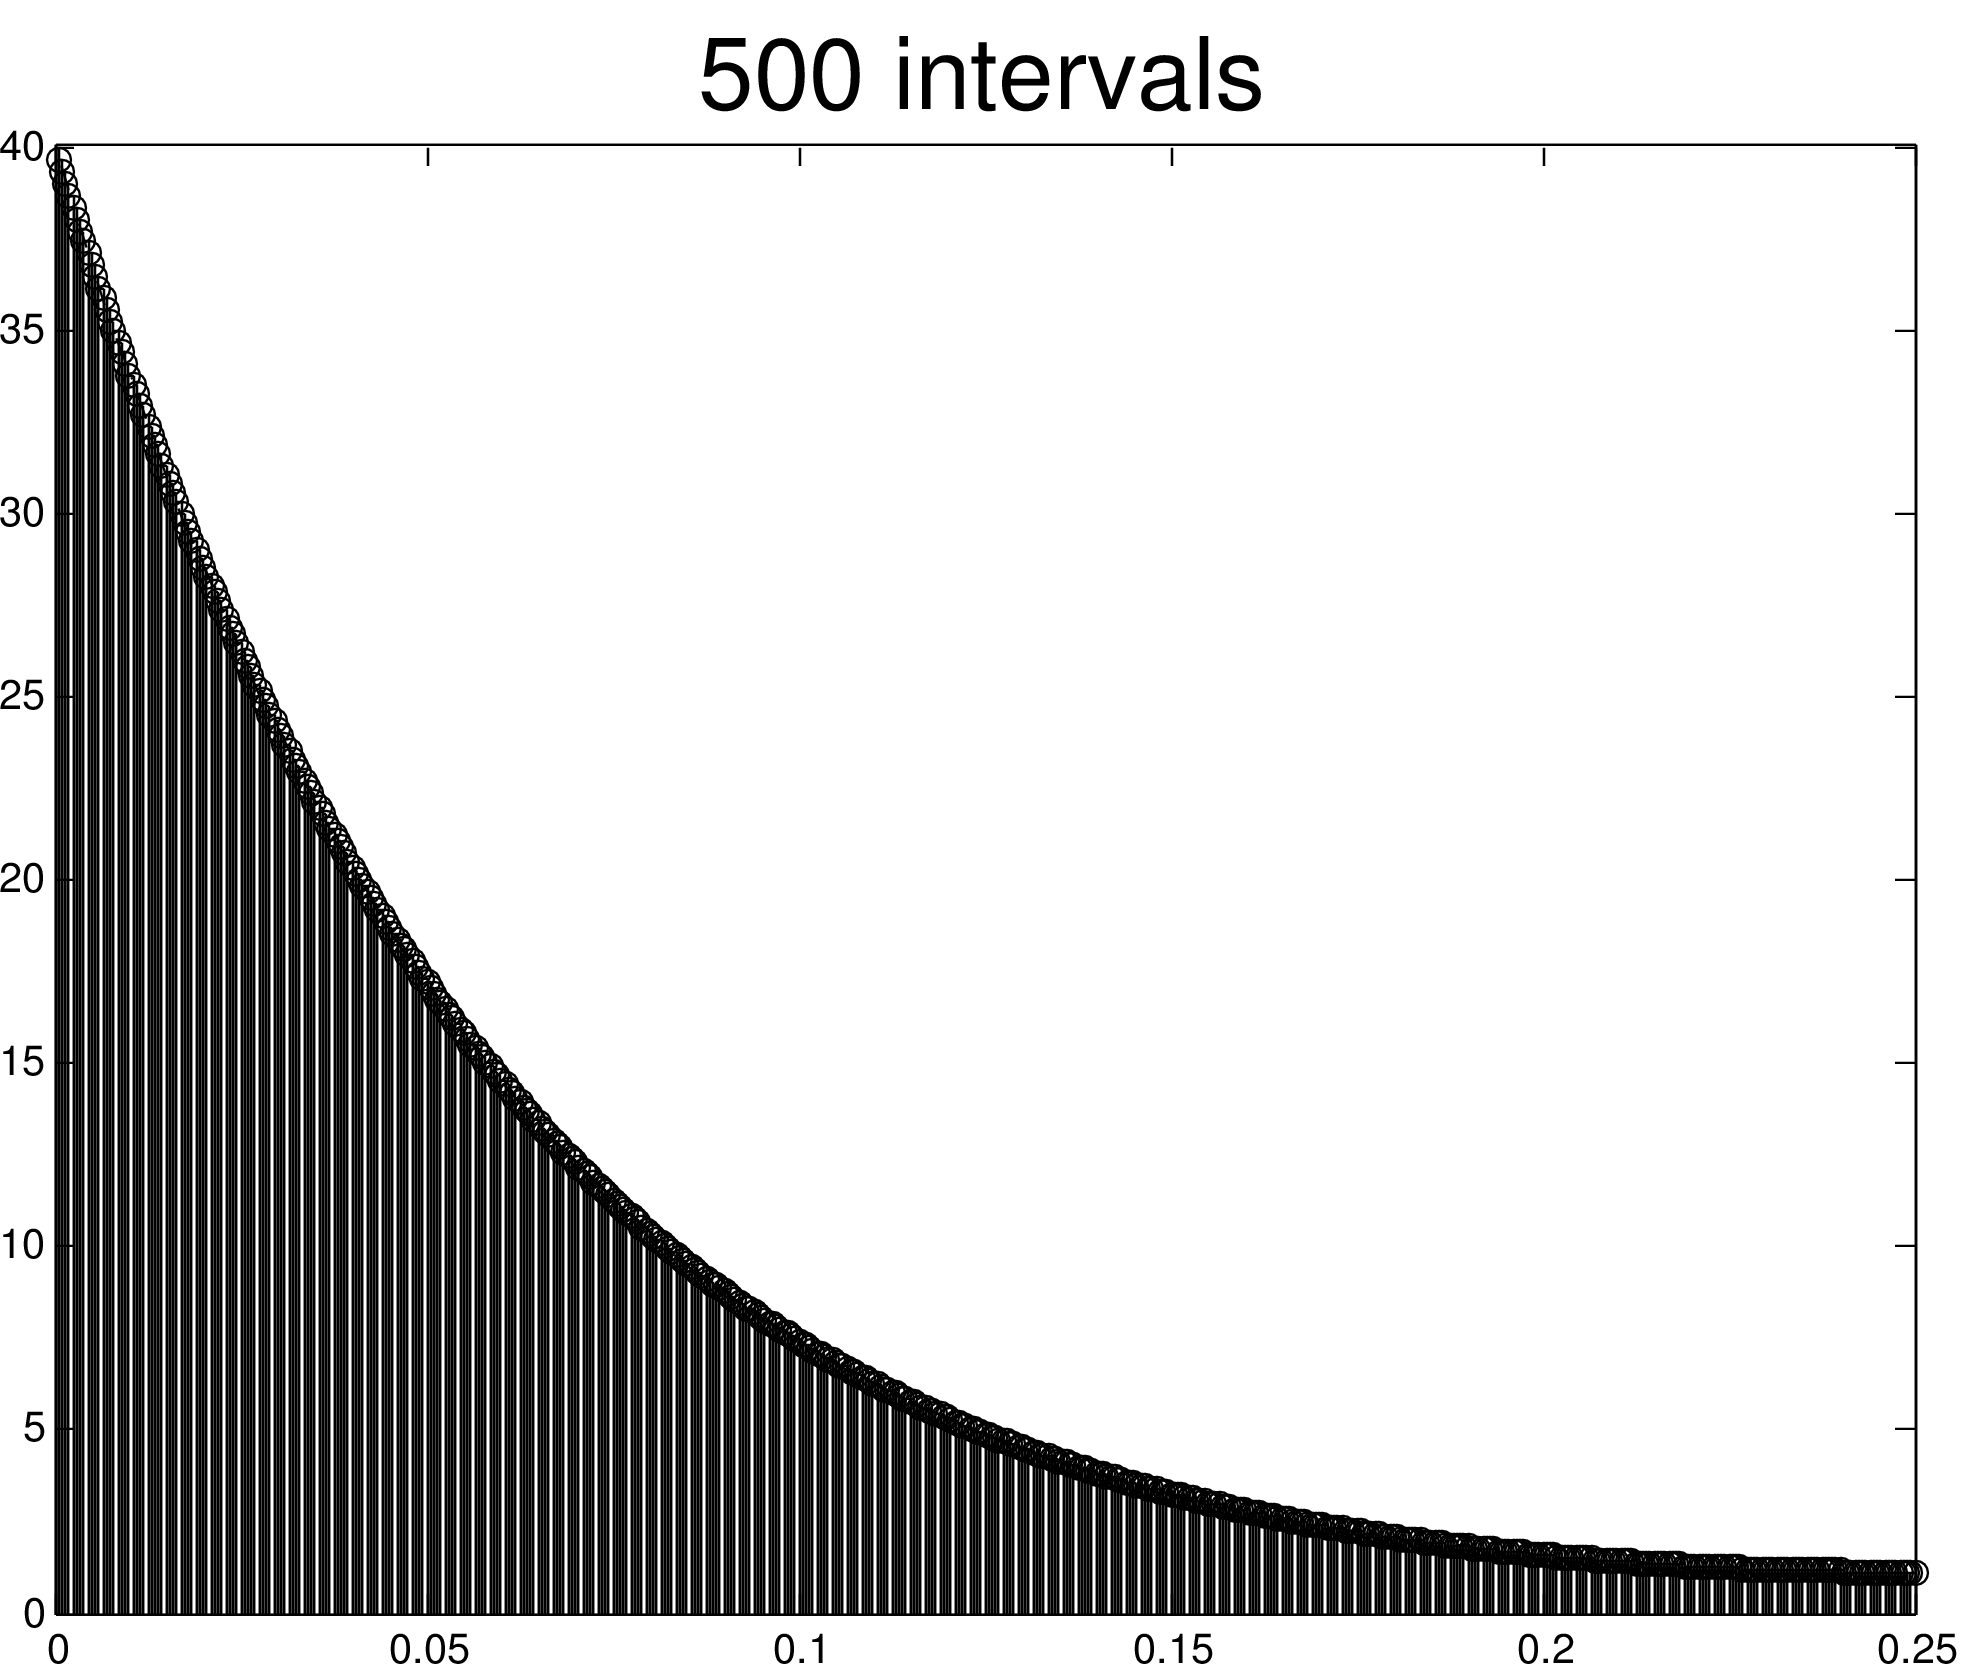
\includegraphics[height=6cm]{graphics/notes_06_f_lhr_500_intervals}
\end{center}
By using enough panels, we can reduce the error to any level we like,
but then it takes longer to compute.

Our real question should be: as we do {\bf more work}, how much {\bf
  more accurate} does our answer become?

\newpage

\problem Download the file \texttt{W7\_1.m}, and extend it so it
  plots the graph of the temperature along the fin.

\vsc

\problem Estimate the integral $\ds Q = \int_0^L h P ~T(x) ~dx$ with
  the left-hand rule,
$$ Q \approx \sum_{i=1}^n h P ~T(x_i)~ \Delta x$$

\vsc

\problem Repeat the calculation, but using the \texttt{sum} command
instead of a loop.  Loops tend to be slow in MATLAB, compared to 
built-in matrix operations.

\vsc

\newpage

\problem Add a print statement that shows the number of intervals
  used, and the resulting error.  Experiment by doubling the number of
  intervals and seeing the resultant reduction in error.

\vsc

\problem Doubling the number of panels does what to the error?

\vfill

\newpage

% \problem Generate a plot of the number of intervals vs. the error.}

% \vsc

% \problem How can you modify the graph of number of panels vs.
%   error to show that the error is in fact being halved every time you
%   double the number of intervals?}

% \vfill
% \vfill

We now have a procedure for estimating integrals {\bf without} needing
to actually use any calculus.  Our next quest will be to make these
integral estimates as {\em accurate} as possible for the {\em least
  amount of work}.  In other words, we will be looking for more {\bf
  efficient} methods.

\newpage

\topic*{Built-In Integration in MATLAB }
\subsection*{Built-In Integration in MATLAB }

\problem Look up the function \texttt{quad} or \texttt{integral} in MATLAB help.

\vsc

\problem Use \texttt{quad} on our sawtooth function and print the error.

\vsc

\problem Experiment with the options for \texttt{quad} to reduce the
  error further.

\vsc

\problem Comment on the error you ask for and the error you get.

\vfill


\newpage

\topic{Numerical Integration in MATLAB - Examples}
\subsection*{Numerical Integration in MATLAB - Examples}



\newpage


\end{document}

